\chapter{System Description}
\label{system_description}

\section{Components of the System}
\label{systemcomponents}
%
\begin{table}[]
\centering
\begin{adjustbox}{max width=\textwidth}
\begin{tabular}{c|c|c|c|c|c|c|c|c}
Part & Component & Length & Diameter & Material & $\epsilon$ & $\Delta z$& Fittings   & $\Sigma k_f$  \\\hline
Ring & $C_4$ 	 & 5m+0.3m& 20 mm 	 & 25 mm PEM& 0.01 mm 	 & 0 m 		 & b,c,c,a,a  &  4.42  		  \\ % Ring
 	 & $C_8$ 	 & 10 m	  & 20 mm 	 & 25 mm PEM& 0.01 mm 	 & 0 m 	 	 & c,b,a,c,b  &  3.92  		  \\
 	 & $C_9$ 	 & 10 m	  & 20 mm 	 & 25 mm PEM& 0.01 mm 	 & 0 m 		 & c 	      &  0.51 		  \\
	 & $C_{10}$  & 10 m	  & 20 mm 	 & 25 mm PEM& 0.01 mm 	 & 0 m 		 & c,a,a 	  &  3.11 		  \\
 	 & $C_{11}$  & 10 m	  & 20 mm 	 & 25 mm PEM& 0.01 mm 	 & 0 m 		 & c,a 		  &  1.81 		  \\
 	 & $C_{12}$  & 10 m	  & 20 mm 	 & 25 mm PEM& 0.01 mm 	 & 0 m 		 & c,c,a,c,b  &  3.63		  \\
 	 & $C_{13}$  & 10 m   & 20 mm 	 & 25 mm PEM& 0.01 mm 	 & 0 m 		 & c 		  &  0.51		  \\
 	 & $C_{14}$  & 5m+4m  & 20 mm 	 & 25 mm PEM& 0.01 mm 	 & 0 m 		 & a,c 		  &  1.81  		  \\ \hline
PMA1 & $C_{19}$	 & 2 m 	  & 10 mm    & 15 mm PEX& 0.007 mm   & 0 m 		 & b,c,d,c,e,a&  3.57 		  \\ % PMA 1 section
	 & $C_{21}$  & 1 m 	  & 10 mm    & 15 mm PEX& 0.007 mm   & 0 m 		 & c,d,b 	  &  1.46 		  \\
 	 & $C_{22}$  & 1 m 	  & 10 mm    & 15 mm PEX& 0.007 mm   & 0 m 		 & c,d,b,e,b  &  7.68  		  \\
 	 & $C_{23}$  & 2 m 	  & 10 mm    & 15 mm PEX& 0.007 mm   & 0 m 		 & a,b,d,e    &  2.55  		  \\ \hline
PMA2 & $C_{23}$  & 3 m	  & 10 mm    & 15 mm PEX& 0.007 mm   & 0.5 m  	 & d,c,a,c,e  &  2.77	      \\
 	 & $C_{23}$  & 1 m 	  & 10 mm    & 15 mm PEX& 0.007 mm   & 0 m 		 & c,e 		  &  0.81    	  \\
 	 & $C_{23}$  & 1 m 	  & 10 mm    & 15 mm PEX& 0.007 mm   & 0 m 	   	 & b,d,c,b 	  &  2.26     	  \\
 	 & $C_{23}$  & 2 m 	  & 10 mm    & 15 mm PEX& 0.007 mm   & 0 m 		 & b,a 		  &  2.10    	  \\ \hline
- 	 & $C_{42}$  & 2 m    & 10 mm 	 & 15 mm PEX& 0.007 mm   & 0.5 m 	 & c,c,a,d,e  &  2.77 		  \\
- 	 &  &  &  &  &  &  &    \\
- 	 &  &  &  &  &  &  &   
\end{tabular}
\end{adjustbox}
\caption{Table with details about the pipes in the water system, shown on \figref{systemdiagram}. Note that $\Sigma k_f$ is an initial guess for the parameter estimation in \secref{SubSecEstimation}.}
\label{tab:pip_detail}
\end{table}


\begin{table}[]
\centering
\begin{tabular}{l|l|l}
Fitting 									  & Symbol 	  & $k_f$   \\ \hline
Tee - Over all loss							  & $k_{f,a}$ & 1.3 	\\
Tee - Straigh through						  & $k_{f,b}$ & 0.8 	\\
$90^\circ$ bend - Diameter/radious ration 1:1 & $k_{f,c}$ & 0.51	\\
Sudden enlarger - Diameter ratio 1:2		  & $k_{f,d}$ & 0.15	\\
Sudden contractor - Diameter ratio 1:2		  & $k_{f,e}$ & 0.3 	
\end{tabular}
\caption{Table with details about the fittings in the water system. The finttings are not shown in \figref{systemdiagram}. The values are found in \citep{Polypipe} and \citep{PEPS}.}
\label{tab:pip_detail}
\end{table}


\begin{table}[]
\centering
\begin{tabular}{c|c|c|c|c|c|c|c}
Part & Component 		& Valve fitting 	& $k_{vs}$  & $n_{gl}$  & $\theta_{off}$ & $\theta_{max}$ & Valve motor 	 \\ \hline
PMA1 & $C_{20}, C_{24}$ & Belimo R2015-1-S1 & 1 		& 3.2 		& $15^\circ$	 & $90^\circ$ 	  & Belimo LRQ24A-SR \\
PMA2 & $C_{27}, C_{31}$ & Belimo R2015-1-S1 & 1 		& 3.2 		& $15^\circ$   	 & $90^\circ$ 	  & Belimo LRQ24A-SR
\end{tabular}
\caption{Table with details about the valves in the water system, shown on \figref{systemdiagram}. The parameters are found in \citep{Belimo1, Belimo2}}
\label{tab:pip_detail}
\end{table}


\begin{table}[]
\centering
\begin{tabular}{c|c|c|c}
Part 	 & Component    		  & Pump type 					 	& Constants 	    \\ \hline
Ring     & $C_2,C_{16}$ 		  & Grundfors UPMXL GEO 25-125 180  & $a_{h0}$ = 1.2024 \\
		 &				 		  &								 	& $a_{h1}$ = 0.0098 \\
		 &						  &								 	& $a_{h2}$ = 0.0147 \\
		 &						  &								 	& $B_{0}$ = 9.8924  \\ \hline 
PMA(1,2) & $C_{18},C_{25},C_{32}$ & Grundfors UPM2 25-60 180	    & $a_{h0}$ = 0.6921 \\
		 &				 		  &								 	& $a_{h1}$ = -0.0177\\
		 &						  &								 	& $a_{h2}$ = 0.0179 \\
		 &						  &								 	& $B_{0}$ = 0.0698  \\
\end{tabular}
\caption{Table with details about the pumps in the water system, shown on \figref{systemdiagram}. The parameters are provided by Grundfos.
\label{tab:pip_detail}
\end{table}


\pagebreak


\section{System Topology}

% \begin{figure}[H]
%   \centering
%   % \begin{minipage}[b]{0.45\textwidth}
%   %   \centering
%   %  % \tikzsetnextfilename{basic_example_sys}
%   %   \tikzset{pressure/.style={draw, circle, inner sep=0pt, text width=4mm, align=center}}
\tikzset{difpres/.style={draw, circle, inner sep=0pt, text width=5mm, align=center}}
\tikzset{connect/.style={draw,circle, inner sep=0pt, text width=2mm, align=center,fill=black}}
\tikzset{evalve/.style={draw, circle, inner sep=0pt, text width=3mm, align=center}}
\begin{tikzpicture} [scale=0.7,transform shape]
%Pump
\begin{scope} [rotate around={90:(0,1)}, shift={(0,1)}]
\draw[transform shape] (0,0) circle (0.5);
\draw[transform shape] (0.5,0) -- (0,0.5);
\draw[transform shape] (0.5,0) -- (0,-0.5);
\end{scope}

%man-valve
\node(n1) at (0.25,3.5) {};
\node(n2) at (-0.25,3.5) {};
\node(n3) at (0.25,2.5) {};
\node(n4) at (-0.25,2.5) {};
\node(n5) at (0,3) {};
\node(n6) at (-0.5,3.25) {};
\node(n7) at (-0.5,2.75) {};
\draw(n1.center)--(n2.center)--(n3.center)--(n4.center)--(n1.center)--(n2.center);
\draw(n5.center)-|(n6.center)--(n7.center);

%elec-valve
\node(n1) at (4.25,3.5) {};
\node(n2) at (3.75,3.5) {};
\node(n3) at (4.25,2.5) {};
\node(n4) at (3.75,2.5) {};
\node(n5) at (4,3) {};
\node[evalve] (n6) at (3.5,3) {};
\draw(n1.center)--(n2.center)--(n3.center)--(n4.center)--(n1.center)--(n2.center);
\draw(n5.center)--(n6);

%man-valve
\node(n1) at (0.25,-0.5) {};
\node(n2) at (-0.25,-0.5) {};
\node(n3) at (0.25,-1.5) {};
\node(n4) at (-0.25,-1.5) {};
\node(n5) at (0,-1) {};
\node(n6) at (-0.5,-0.75) {};
\node(n7) at (-0.5,-1.25) {};
\draw(n1.center)--(n2.center)--(n3.center)--(n4.center)--(n1.center)--(n2.center);
\draw(n5.center)-|(n6.center)--(n7.center);

%man-valve
%\draw[very thick](-0.25,-1) -- (0.25,-1) -- (-0.25,-2) -- (0.25,-2) -- (-0.25,-1) -- (0.25,-1);
%\draw[very thick](0,-1.5) -- (-0.5,-1.5);
%\draw[very thick](-0.5,-1.25) -- (-0.5,-1.75);

%GND
\draw(-0.3,-2.5)--(0.3,-2.5);
\draw(-0.15,-2.6)--(0.15,-2.6);

%GND
\draw(3.7,1.5)--(4.3,1.5);
\draw(3.85,1.4)--(4.15,1.4);

%pipe
%right arcs
\draw (2.5,5.5) arc (90:-90:0.05);
\draw (2.5,5.3) arc (90:-90:0.05);
\draw (2.5,5.1) arc (90:-90:0.05);
%left arcs
\draw (1,5.4) arc (90:270:0.05);
\draw (1,5.2) arc (90:270:0.05);
\draw (1,5) arc (90:270:0.05);
%lines
\draw(1,5.5) -- (2.5,5.5);
\draw(1,5.4) -- (2.5,5.4);
\draw(1,5.3) -- (2.5,5.3);
\draw(1,5.2) -- (2.5,5.2);
\draw(1,5.1) -- (2.5,5.1);
\draw(1,5) -- (2.5,5);
\draw[rounded corners](1,4.9) -- (2.65,4.9) -- (2.65,5.5) -- (3.4,5.5);
%pipe name
%\node at (2,4) {$\text{C}_1$};

%pressure sensor
\node[connect] (PD1) at (3.5,5.5) {};
\node(P1) at ($(PD1)+(0,1)$) [pressure] {P};
\draw(PD1) -- (P1);

%differential pressure sensor
\node[connect] (CDP1) at (0,4) {};
\node[connect] (CDP2) at (0,-2) {};
\node[difpres] (DP1) at (-1.5,0.5) {DP};
\draw(CDP1) -| (DP1)  |- (CDP2);

%Connections
\draw(0,1.5) -- (0,2.5);
\draw(0,0.5) -- (0,-0.5);
\draw(0,-1.5) -- (0,-2.5);
\draw[rounded corners](0,3.5)--(0,5.5)--(1,5.5);
\draw[rounded corners](3,5.5)--(4,5.5)--(4,3.5);
\draw(4,2.5) -- (4,1.5);

\end{tikzpicture}

     
%   %   \caption{Basic water distribution network.}
%   %   \label{fig:Basic_example_sys}
%   % \end{minipage}
%   % \hspace{15pt}
%   \begin{minipage}[b]{0.45\textwidth}
%     \begin{tabular}{|c|c|} \hline
%       \bfseries Symbol                                                         & \bfseries Name                \\ \hline
%       %\tikzsetnextfilename{pump}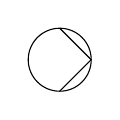
\begin{tikzpicture}[scale=0.8,transform shape]
%Pump
\draw (0,0) circle (0.5);
\draw (0.5,0) -- (0,0.5);
\draw (0.5,0) -- (0,-0.5);
\addvmargin{4mm}
\end{tikzpicture}

                           & Pump                          \\ \hline
%       %\tikzsetnextfilename{manual_valve}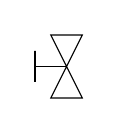
\begin{tikzpicture}[scale=0.8,transform shape]
%man-valve
\node(n1) at (0.25,2) {};
\node(n2) at (-0.25,2) {};
\node(n3) at (0.25,1) {};
\node(n4) at (-0.25,1) {};
\node(n5) at (0,1.5) {};
\node(n6) at (-0.5,1.75) {};
\node(n7) at (-0.5,1.25) {};
\draw(n1.center)--(n2.center)--(n3.center)--(n4.center)--(n1.center)--(n2.center);
\draw(n5.center)-|(n6.center)--(n7.center);
\addvmargin{4mm}
\end{tikzpicture}

           & Manual valve                  \\ \hline
%       \begin{figure}\tikzsetnextfilename{elec_valve}\tikzset{evalve/.style={draw, circle, inner sep=0pt, text width=3mm, align=center}}
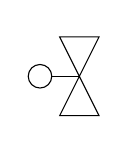
\begin{tikzpicture}
%elec-valve
\node(n1) at (4.25,2) {};
\node(n2) at (3.75,2) {};
\node(n3) at (4.25,1) {};
\node(n4) at (3.75,1) {};
\node(n5) at (4,1.5) {};
\node(n6) at (3.5,1.5) [evalve] {};
\draw(n1.center)--(n2.center)--(n3.center)--(n4.center)--(n1.center)--(n2.center);
\draw(n5.center)--(n6);
\addvmargin{4mm}
\end{tikzpicture}

    \end{figure}           & Electronic valve              \\ \hline
%       %\tikzsetnextfilename{pipe}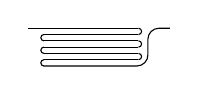
\begin{tikzpicture}[scale=0.8,transform shape]
%pipe
%right arcs
\draw (2.5,3.5) arc (90:-90:0.05);
\draw (2.5,3.3) arc (90:-90:0.05);
\draw (2.5,3.1) arc (90:-90:0.05);
%left arcs
\draw (1,3.4) arc (90:270:0.05);
\draw (1,3.2) arc (90:270:0.05);
\draw (1,3) arc (90:270:0.05);
%lines
\draw(0.75,3.5) -- (2.5,3.5);
\draw(1,3.4) -- (2.5,3.4);
\draw(1,3.3) -- (2.5,3.3);
\draw(1,3.2) -- (2.5,3.2);
\draw(1,3.1) -- (2.5,3.1);
\draw(1,3) -- (2.5,3);
\draw[rounded corners](1,2.9) -- (2.65,2.9) -- (2.65,3.5) -- (3,3.5);
\addvmargin{4mm}
\end{tikzpicture}

                           & Pipe segment                  \\ \hline
%       %\tikzsetnextfilename{pressure_sensor}\tikzset{pressure/.style={draw, circle, inner sep=0pt, text width=4mm, align=center}}
\tikzset{difpres/.style={draw, circle, inner sep=0pt, text width=5mm, align=center}}
\tikzset{connect/.style={draw,circle, inner sep=0pt, text width=2mm, align=center,fill=black}}
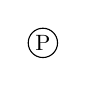
\begin{tikzpicture}[scale=0.8,transform shape]
%pressure sensor
\node(P1) at (0,0) [pressure] {P};
\addvmargin{4mm}
\end{tikzpicture}

     & Pressure sensor              \\ \hline
%       %\tikzsetnextfilename{dif_pres_sens}\tikzset{pressure/.style={draw, circle, inner sep=0pt, text width=4mm, align=center}}
\tikzset{difpres/.style={draw, circle, inner sep=0pt, text width=5mm, align=center}}
\tikzset{connect/.style={draw,circle, inner sep=0pt, text width=2mm, align=center,fill=black}}

\begin{tikzpicture}[scale=0.8,transform shape]
%differential pressure sensor
\node(DP1) at (-2,0) [difpres] {DP};
\addvmargin{4mm}
\end{tikzpicture}

         & Differential pressure sensor  \\ \hline
%       %\tikzsetnextfilename{gnd}\begin{tikzpicture}[scale=0.8,transform shape]
%GND
\draw(-0.3,-2.5)--(0.3,-2.5);
\draw(-0.15,-2.6)--(0.15,-2.6);
\draw(0,-2.5)--(0,-2);
\addvmargin{4mm}
\end{tikzpicture}

                             & Gnd                           \\ \hline
%     \end{tabular}
%     \captionof{table}{Symbol and name for component in the water network.}  
%     \label{tab:sys_comp_overview}
%   \end{minipage}
% \end{figure}


\label{systemdiagram}
%tikz of system diagram
\begin{figure}[H]
\centering
\resizebox{0.75\linewidth}{!}{\tikzset{pressure/.style={draw, circle, inner sep=0pt, text width=5mm, align=center}}
\tikzset{difpres/.style={draw, circle, inner sep=0pt, text width=6mm, align=center}}
\tikzset{connect/.style={draw,circle, inner sep=0pt, text width=2mm, align=center,fill=black}}
\tikzset{evalve/.style={draw, circle, inner sep=0pt, text width=3mm, align=center}}
\begin{turn}{90}
\begin{tikzpicture}



%Pump north
\node[draw,circle,minimum size=1cm] (p0) at (6,6) {};
\node(p1) at ($(p0)+(-0.5,0)$) {};
\node(p2) at ($(p1)+(0.5,0.5)$) {};
\node(p3) at ($(p1)+(1,0)$) {};
\draw(p1.center) -- (p2.center) -- (p3.center);
\node at ($(p1)+(1.5,0)$) {\Large $C_{18}$};

%Pump north
\node[draw,circle,minimum size=1cm] (p0) at (-5,9) {};
\node(p1) at ($(p0)+(-0.5,0)$) {};
\node(p2) at ($(p1)+(0.5,0.5)$) {};
\node(p3) at ($(p1)+(1,0)$) {};
\draw(p1.center) -- (p2.center) -- (p3.center);
\node at ($(p1)+(1.5,0)$) {\Large $C_{32}$};

%Pump north
\node[draw,circle,minimum size=1cm] (p0) at (20,6) {};
\node(p1) at ($(p0)+(-0.5,0)$) {};
\node(p2) at ($(p1)+(0.5,0.5)$) {};
\node(p3) at ($(p1)+(1,0)$) {};
\draw(p1.center) -- (p2.center) -- (p3.center);
\node at ($(p1)+(1.5,0)$) {\Large $C_{25}$};

%Pump north
\node[draw,circle,minimum size=1cm] (p0) at (-1.5,0.5) {};
\node(p1) at ($(p0)+(-0.5,0)$) {};
\node(p2) at ($(p1)+(0.5,0.5)$) {};
\node(p3) at ($(p1)+(1,0)$) {};
\draw(p1.center) -- (p2.center) -- (p3.center);
\node at ($(p1)+(1.5,0)$) {\Large $C_{2}$};

%Pump north
\node[draw,circle,minimum size=1cm] (p0) at (28,0.5) {};
\node(p1) at ($(p0)+(-0.5,0)$) {};
\node(p2) at ($(p1)+(0.5,0.5)$) {};
\node(p3) at ($(p1)+(1,0)$) {};
\draw(p1.center) -- (p2.center) -- (p3.center);
\node at ($(p1)+(1.5,0)$) {\Large $C_{16}$};

%man-valve
\node(n1) at (6.25,5) {};
\draw(n1.center) -- ($(n1)-(0.5,0)$) --
($(n1)-(0,1)$) -- ($(n1)-(0.5,1)$) --  (n1.center);
\draw($(n1)-(0.75,0.25)$) -- ($(n1)-(0.75,0.75)$) -- 
($(n1)-(0.75,0.5)$) --  ($(n1)-(0.25,0.5)$);
%\node at ($(n1)+(0.5,-0.5)$) {\Large $C_{18d}$};

%man-valve
\node(n1) at (6.25,8) {};
\draw(n1.center) -- ($(n1)-(0.5,0)$) --
($(n1)-(0,1)$) -- ($(n1)-(0.5,1)$) --  (n1.center);
\draw($(n1)-(0.75,0.25)$) -- ($(n1)-(0.75,0.75)$) -- 
($(n1)-(0.75,0.5)$) --  ($(n1)-(0.25,0.5)$);
%\node at ($(n1)+(0.5,-0.5)$) {\Large $C_{18u}$};

%man-valve
\node(n1) at (20.25,8) {};
\draw(n1.center) -- ($(n1)-(0.5,0)$) --
($(n1)-(0,1)$) -- ($(n1)-(0.5,1)$) --  (n1.center);
\draw($(n1)-(0.75,0.25)$) -- ($(n1)-(0.75,0.75)$) -- 
($(n1)-(0.75,0.5)$) --  ($(n1)-(0.25,0.5)$);
%\node at ($(n1)+(0.5,-0.5)$) {\Large $C_{25u}$};

%man-valve
\node(n1) at (20.25,5) {};
\draw(n1.center) -- ($(n1)-(0.5,0)$) --
($(n1)-(0,1)$) -- ($(n1)-(0.5,1)$) --  (n1.center);
\draw($(n1)-(0.75,0.25)$) -- ($(n1)-(0.75,0.75)$) -- 
($(n1)-(0.75,0.5)$) --  ($(n1)-(0.25,0.5)$);
%\node at ($(n1)+(0.5,-0.5)$) {\Large $C_{25d}$};

%man-valve
\node(n1) at (-1.25,2.5) {};
\draw(n1.center) -- ($(n1)-(0.5,0)$) --
($(n1)-(0,1)$) -- ($(n1)-(0.5,1)$) --  (n1.center);
\draw($(n1)-(0.75,0.25)$) -- ($(n1)-(0.75,0.75)$) -- 
($(n1)-(0.75,0.5)$) --  ($(n1)-(0.25,0.5)$);
%\node at ($(n1)+(0.4,-0.5)$) {\Large $C_{3}$};

%man-valve
\node(n1) at (-1.25,-0.5) {};
\draw(n1.center) -- ($(n1)-(0.5,0)$) --
($(n1)-(0,1)$) -- ($(n1)-(0.5,1)$) --  (n1.center);
\draw($(n1)-(0.75,0.25)$) -- ($(n1)-(0.75,0.75)$) -- 
($(n1)-(0.75,0.5)$) --  ($(n1)-(0.25,0.5)$);
%\node at ($(n1)+(0.4,-0.5)$) {\Large $C_{1}$};

%man-valve
\node(n1) at (-4.75,11.5) {};
\draw(n1.center) -- ($(n1)-(0.5,0)$) --
($(n1)-(0,1)$) -- ($(n1)-(0.5,1)$) --  (n1.center);
\draw($(n1)-(0.75,0.25)$) -- ($(n1)-(0.75,0.75)$) -- 
($(n1)-(0.75,0.5)$) --  ($(n1)-(0.25,0.5)$);
%\node at ($(n1)+(0.5,-0.5)$) {\Large $C_{6}$};

%man-valve
\node(n1) at (-4.75,7.5) {};
\draw(n1.center) -- ($(n1)-(0.5,0)$) --
($(n1)-(0,1)$) -- ($(n1)-(0.5,1)$) --  (n1.center);
\draw($(n1)-(0.75,0.25)$) -- ($(n1)-(0.75,0.75)$) -- 
($(n1)-(0.75,0.5)$) --  ($(n1)-(0.25,0.5)$);
%\node at ($(n1)+(0.5,-0.5)$) {\Large $C_{5}$};

%man-valve
\node(n1) at (28.25,-0.5) {};
\draw(n1.center) -- ($(n1)-(0.5,0)$) --
($(n1)-(0,1)$) -- ($(n1)-(0.5,1)$) --  (n1.center);
\draw($(n1)-(0.75,0.25)$) -- ($(n1)-(0.75,0.75)$) -- 
($(n1)-(0.75,0.5)$) --  ($(n1)-(0.25,0.5)$);
%\node at ($(n1)+(0.5,-0.5)$) {\Large $C_{17}$};

%man-valve
\node(n1) at (28.25,2.5) {};
\draw(n1.center) -- ($(n1)-(0.5,0)$) --
($(n1)-(0,1)$) -- ($(n1)-(0.5,1)$) --  (n1.center);
\draw($(n1)-(0.75,0.25)$) -- ($(n1)-(0.75,0.75)$) -- 
($(n1)-(0.75,0.5)$) --  ($(n1)-(0.25,0.5)$);
%\node at ($(n1)+(0.5,-0.5)$) {\Large $C_{15}$};

%elec-valve
\node(n1) at (10.25,11.5) {};
\draw(n1.center) -- ($(n1)-(0.5,0)$) --
($(n1)-(0,1)$) -- ($(n1)-(0.5,1)$) --  (n1.center);
\draw($(n1)-(0.75,0.5)$) circle (1.5mm); 
\draw($(n1)-(0.6,0.5)$)--  ($(n1)-(0.25,0.5)$);
\node at ($(n1)+(0.3,-0.5)$) {\Large $C_{24}$};

%elec-valve
\node(n1) at (-1.25,11.5) {};
\draw(n1.center) -- ($(n1)-(0.5,0)$) --
($(n1)-(0,1)$) -- ($(n1)-(0.5,1)$) --  (n1.center);
\draw($(n1)-(0.75,0.5)$) circle (1.5mm); 
\draw($(n1)-(0.6,0.5)$)--  ($(n1)-(0.25,0.5)$);
\node at ($(n1)+(0.3,-0.5)$) {\Large $C_{20}$};

%elec-valve
\node(n1) at (24.25,11.5) {};
\draw(n1.center) -- ($(n1)-(0.5,0)$) --
($(n1)-(0,1)$) -- ($(n1)-(0.5,1)$) --  (n1.center);
\draw($(n1)-(0.75,0.5)$) circle (1.5mm); 
\draw($(n1)-(0.6,0.5)$)--  ($(n1)-(0.25,0.5)$);
\node at ($(n1)+(0.3,-0.5)$) {\Large $C_{31}$};

%elec-valve
\node(n1) at (13.25,11.5) {};
\draw(n1.center) -- ($(n1)-(0.5,0)$) --
($(n1)-(0,1)$) -- ($(n1)-(0.5,1)$) --  (n1.center);
\draw($(n1)-(0.75,0.5)$) circle (1.5mm); 
\draw($(n1)-(0.6,0.5)$)--  ($(n1)-(0.25,0.5)$);
\node at ($(n1)+(0.3,-0.5)$) {\Large $C_{27}$};

%man-valve
%\draw[very thick](-0.25,-1) -- (0.25,-1) -- (-0.25,-2) -- (0.25,-2) -- (-0.25,-1) -- (0.25,-1);
%\draw[very thick](0,-1.5) -- (-0.5,-1.5);
%\draw[very thick](-0.5,-1.25) -- (-0.5,-1.75);


%GND
\node(g1) at (-1.5,-2.5) {};
\draw(g1.center) -- ($(g1)+(0.3,0)$) -- ($(g1)-(0.3,0)$);
\draw($(g1)-(0.15,0.1)$) -- ($(g1)+(0.15,-0.1)$);

%GND
\node(g1) at (-1.5,9.5) {};
\draw(g1.center) -- ($(g1)+(0.3,0)$) -- ($(g1)-(0.3,0)$);
\draw($(g1)-(0.15,0.1)$) -- ($(g1)+(0.15,-0.1)$);

%GND
\node(g1) at (28,-2.5) {};
\draw(g1.center) -- ($(g1)+(0.3,0)$) -- ($(g1)-(0.3,0)$);
\draw($(g1)-(0.15,0.1)$) -- ($(g1)+(0.15,-0.1)$);

%GND
\node(g1) at (13,9.5) {};
\draw(g1.center) -- ($(g1)+(0.3,0)$) -- ($(g1)-(0.3,0)$);
\draw($(g1)-(0.15,0.1)$) -- ($(g1)+(0.15,-0.1)$);

%GND
\node(g1) at (24,9.5) {};
\draw(g1.center) -- ($(g1)+(0.3,0)$) -- ($(g1)-(0.3,0)$);
\draw($(g1)-(0.15,0.1)$) -- ($(g1)+(0.15,-0.1)$);

%GND
\node(g1) at (10,9.5) {};
\draw(g1.center) -- ($(g1)+(0.3,0)$) -- ($(g1)-(0.3,0)$);
\draw($(g1)-(0.15,0.1)$) -- ($(g1)+(0.15,-0.1)$);


%pipe
\node(r1) at (12,3) {};
\draw (r1.center) -- ($(r1)+(1.5,0)$) arc (90:-90:0.05) -- 
($(r1)+(0,-0.1)$) arc (90:270:0.05) --
($(r1)+(1.5,-0.2)$) arc (90:-90:0.05) --
($(r1)+(0,-0.3)$) arc (90:270:0.05) --
($(r1)+(1.5,-0.4)$) arc (90:-90:0.05) --
($(r1)+(0,-0.5)$) arc (90:270:0.05);
\draw[rounded corners] ($(r1)+(0,-0.6)$) -- 
($(r1)+(1.65,-0.6)$) -- ($(r1)+(1.65,0)$) -- ($(r1)+(2.5,0)$);
\node at ($(r1)+(0.75,-1)$) {\Large $C_{9},C_{10}$};

%pipe
\node(r1) at (12,-1) {};
\draw (r1.center) -- ($(r1)+(1.5,0)$) arc (90:-90:0.05) -- 
($(r1)+(0,-0.1)$) arc (90:270:0.05) --
($(r1)+(1.5,-0.2)$) arc (90:-90:0.05) --
($(r1)+(0,-0.3)$) arc (90:270:0.05) --
($(r1)+(1.5,-0.4)$) arc (90:-90:0.05) --
($(r1)+(0,-0.5)$) arc (90:270:0.05);
\draw[rounded corners] ($(r1)+(0,-0.6)$) -- 
($(r1)+(1.65,-0.6)$) -- ($(r1)+(1.65,0)$) -- ($(r1)+(2.5,0)$);
\node at ($(r1)+(0.75,-1)$) {\Large $C_{12},C_{13}$};

%pipe
\node(r1) at (12,16.5) {};
\draw (r1.center) -- ($(r1)+(1.5,0)$) arc (90:-90:0.05) -- 
($(r1)+(0,-0.1)$) arc (90:270:0.05) --
($(r1)+(1.5,-0.2)$) arc (90:-90:0.05) --
($(r1)+(0,-0.3)$) arc (90:270:0.05) --
($(r1)+(1.5,-0.4)$) arc (90:-90:0.05) --
($(r1)+(0,-0.5)$) arc (90:270:0.05);
\draw[rounded corners] ($(r1)+(0,-0.6)$) -- 
($(r1)+(1.65,-0.6)$) -- ($(r1)+(1.65,0)$) -- ($(r1)+(2.5,0)$);
\node at ($(r1)+(0.75,-1)$) {\Large $C_{42}$};

%pipe
\node(r1) at (25,3) {};
\draw (r1.center) -- ($(r1)+(1.5,0)$) arc (90:-90:0.05) -- 
($(r1)+(0,-0.1)$) arc (90:270:0.05) --
($(r1)+(1.5,-0.2)$) arc (90:-90:0.05) --
($(r1)+(0,-0.3)$) arc (90:270:0.05) --
($(r1)+(1.5,-0.4)$) arc (90:-90:0.05) --
($(r1)+(0,-0.5)$) arc (90:270:0.05);
\draw[rounded corners] ($(r1)+(0,-0.6)$) -- 
($(r1)+(1.65,-0.6)$) -- ($(r1)+(1.65,0)$) -- ($(r1)+(2.5,0)$);
\node at ($(r1)+(0.75,-1)$) {\Large $C_{14}$};

%pipe
\node(r1) at (21.5,3) {};
\draw (r1.center) -- ($(r1)+(1.5,0)$) arc (90:-90:0.05) -- 
($(r1)+(0,-0.1)$) arc (90:270:0.05) --
($(r1)+(1.5,-0.2)$) arc (90:-90:0.05) --
($(r1)+(0,-0.3)$) arc (90:270:0.05) --
($(r1)+(1.5,-0.4)$) arc (90:-90:0.05) --
($(r1)+(0,-0.5)$) arc (90:270:0.05);
\draw[rounded corners] ($(r1)+(0,-0.6)$) -- 
($(r1)+(1.65,-0.6)$) -- ($(r1)+(1.65,0)$) -- ($(r1)+(2.5,0)$);
\node at ($(r1)+(0.75,-1)$) {\Large $C_{11}$};

%pipe
\node(r1) at (6,10) {};
\begin{scope} [rotate around={90:(r1)}]
\draw (r1.center) -- ($(r1)+(1.5,0)$) arc (90:-90:0.05) -- 
($(r1)+(0,-0.1)$) arc (90:270:0.05) --
($(r1)+(1.5,-0.2)$) arc (90:-90:0.05) --
($(r1)+(0,-0.3)$) arc (90:270:0.05) --
($(r1)+(1.5,-0.4)$) arc (90:-90:0.05) --
($(r1)+(0,-0.5)$) arc (90:270:0.05);
\draw[rounded corners] ($(r1)+(0,-0.6)$) -- 
($(r1)+(1.65,-0.6)$) -- ($(r1)+(1.65,0)$) -- ($(r1)+(2.5,0)$);
\end{scope}
\node at ($(r1)+(1.25,0.75)$) {\Large $C_{19}$};

%pipe
\node(r1) at (3,13) {};
\draw (r1.center) -- ($(r1)+(1.5,0)$) arc (90:-90:0.05) -- 
($(r1)+(0,-0.1)$) arc (90:270:0.05) --
($(r1)+(1.5,-0.2)$) arc (90:-90:0.05) --
($(r1)+(0,-0.3)$) arc (90:270:0.05) --
($(r1)+(1.5,-0.4)$) arc (90:-90:0.05) --
($(r1)+(0,-0.5)$) arc (90:270:0.05);
\draw[rounded corners] ($(r1)+(0,-0.6)$) -- 
($(r1)+(1.65,-0.6)$) -- ($(r1)+(1.65,0)$) -- ($(r1)+(2.5,0)$);
\node at ($(r1)+(0.75,-1)$) {\Large $C_{22}$};

%pipe
\node(r1) at (7,13) {};
\draw (r1.center) -- ($(r1)+(1.5,0)$) arc (90:-90:0.05) -- 
($(r1)+(0,-0.1)$) arc (90:270:0.05) --
($(r1)+(1.5,-0.2)$) arc (90:-90:0.05) --
($(r1)+(0,-0.3)$) arc (90:270:0.05) --
($(r1)+(1.5,-0.4)$) arc (90:-90:0.05) --
($(r1)+(0,-0.5)$) arc (90:270:0.05);
\draw[rounded corners] ($(r1)+(0,-0.6)$) -- 
($(r1)+(1.65,-0.6)$) -- ($(r1)+(1.65,0)$) -- ($(r1)+(2.5,0)$);
\node at ($(r1)+(0.75,-1)$) {\Large $C_{23}$};

%pipe
\node(r1) at (3,3) {};
\draw (r1.center) -- ($(r1)+(1.5,0)$) arc (90:-90:0.05) -- 
($(r1)+(0,-0.1)$) arc (90:270:0.05) --
($(r1)+(1.5,-0.2)$) arc (90:-90:0.05) --
($(r1)+(0,-0.3)$) arc (90:270:0.05) --
($(r1)+(1.5,-0.4)$) arc (90:-90:0.05) --
($(r1)+(0,-0.5)$) arc (90:270:0.05);
\draw[rounded corners] ($(r1)+(0,-0.6)$) -- 
($(r1)+(1.65,-0.6)$) -- ($(r1)+(1.65,0)$) -- ($(r1)+(2.5,0)$);
\node at ($(r1)+(0.75,-1)$) {\Large $C_{8}$};

%pipe
\node(r1) at (0,13) {};
\draw (r1.center) -- ($(r1)+(1.5,0)$) arc (90:-90:0.05) -- 
($(r1)+(0,-0.1)$) arc (90:270:0.05) --
($(r1)+(1.5,-0.2)$) arc (90:-90:0.05) --
($(r1)+(0,-0.3)$) arc (90:270:0.05) --
($(r1)+(1.5,-0.4)$) arc (90:-90:0.05) --
($(r1)+(0,-0.5)$) arc (90:270:0.05);
\draw[rounded corners] ($(r1)+(0,-0.6)$) -- 
($(r1)+(1.65,-0.6)$) -- ($(r1)+(1.65,0)$) -- ($(r1)+(2.5,0)$);
\node at ($(r1)+(0.75,-1)$) {\Large $C_{21}$};

%pipe
\node(r1) at (20,10) {};
\begin{scope} [rotate around={90:(r1)}]
\draw (r1.center) -- ($(r1)+(1.5,0)$) arc (90:-90:0.05) -- 
($(r1)+(0,-0.1)$) arc (90:270:0.05) --
($(r1)+(1.5,-0.2)$) arc (90:-90:0.05) --
($(r1)+(0,-0.3)$) arc (90:270:0.05) --
($(r1)+(1.5,-0.4)$) arc (90:-90:0.05) --
($(r1)+(0,-0.5)$) arc (90:270:0.05);
\draw[rounded corners] ($(r1)+(0,-0.6)$) -- 
($(r1)+(1.65,-0.6)$) -- ($(r1)+(1.65,0)$) -- ($(r1)+(2.5,0)$);
\end{scope}
\node at ($(r1)+(1.25,0.75)$) {\Large $C_{26}$};

%pipe
\node(r1) at (14,13) {};
\draw (r1.center) -- ($(r1)+(1.5,0)$) arc (90:-90:0.05) -- 
($(r1)+(0,-0.1)$) arc (90:270:0.05) --
($(r1)+(1.5,-0.2)$) arc (90:-90:0.05) --
($(r1)+(0,-0.3)$) arc (90:270:0.05) --
($(r1)+(1.5,-0.4)$) arc (90:-90:0.05) --
($(r1)+(0,-0.5)$) arc (90:270:0.05);
\draw[rounded corners] ($(r1)+(0,-0.6)$) -- 
($(r1)+(1.65,-0.6)$) -- ($(r1)+(1.65,0)$) -- ($(r1)+(2.5,0)$);
\node at ($(r1)+(0.75,-1)$) {\Large $C_{28}$};

%pipe
\node(r1) at (17,13) {};
\draw (r1.center) -- ($(r1)+(1.5,0)$) arc (90:-90:0.05) -- 
($(r1)+(0,-0.1)$) arc (90:270:0.05) --
($(r1)+(1.5,-0.2)$) arc (90:-90:0.05) --
($(r1)+(0,-0.3)$) arc (90:270:0.05) --
($(r1)+(1.5,-0.4)$) arc (90:-90:0.05) --
($(r1)+(0,-0.5)$) arc (90:270:0.05);
\draw[rounded corners] ($(r1)+(0,-0.6)$) -- 
($(r1)+(1.65,-0.6)$) -- ($(r1)+(1.65,0)$) -- ($(r1)+(2.5,0)$);
\node at ($(r1)+(0.75,-1)$) {\Large $C_{29}$};

%pipe
\node(r1) at (21,13) {};
\draw (r1.center) -- ($(r1)+(1.5,0)$) arc (90:-90:0.05) -- 
($(r1)+(0,-0.1)$) arc (90:270:0.05) --
($(r1)+(1.5,-0.2)$) arc (90:-90:0.05) --
($(r1)+(0,-0.3)$) arc (90:270:0.05) --
($(r1)+(1.5,-0.4)$) arc (90:-90:0.05) --
($(r1)+(0,-0.5)$) arc (90:270:0.05);
\draw[rounded corners] ($(r1)+(0,-0.6)$) -- 
($(r1)+(1.65,-0.6)$) -- ($(r1)+(1.65,0)$) -- ($(r1)+(2.5,0)$);
\node at ($(r1)+(0.75,-1)$) {\Large $C_{30}$};

%pipe
\node(r1) at (-0.5,3) {};
\draw (r1.center) -- ($(r1)+(1.5,0)$) arc (90:-90:0.05) -- 
($(r1)+(0,-0.1)$) arc (90:270:0.05) --
($(r1)+(1.5,-0.2)$) arc (90:-90:0.05) --
($(r1)+(0,-0.3)$) arc (90:270:0.05) --
($(r1)+(1.5,-0.4)$) arc (90:-90:0.05) --
($(r1)+(0,-0.5)$) arc (90:270:0.05);
\draw[rounded corners] ($(r1)+(0,-0.6)$) -- 
($(r1)+(1.65,-0.6)$) -- ($(r1)+(1.65,0)$) -- ($(r1)+(2.5,0)$);
\node at ($(r1)+(0.75,-1)$) {\Large $C_{4}$};

%pressure sensor
\node (PD1) at (-1.5,3) {};
\node(P1) at ($(PD1)+(0,1)$) [pressure] {P};
\draw(PD1.center) -- (P1);

%pressure sensor
\node (PD1) at (23.5,13) {};
\node(P1) at ($(PD1)+(0,1)$) [pressure] {P};
\draw(PD1.center) -- (P1);

%pressure sensor
\node (PD1) at (9.5,13) {};
\node(P1) at ($(PD1)+(0,1)$) [pressure] {P};
\draw(PD1.center) -- (P1);

%pressure sensor
\node (PD1) at (28,3) {};
\node(P1) at ($(PD1)+(0,1)$) [pressure] {P};
\draw(PD1.center) -- (P1);

%pressure sensor
\node (PD1) at (16.5,13) {};
\node(P1) at ($(PD1)+(0,1)$) [pressure] {P};
\draw(PD1.center) -- (P1);

%pressure sensor
\node (PD1) at (2.5,13) {};
\node(P1) at ($(PD1)+(0,1)$) [pressure] {P};
\draw(PD1.center) -- (P1);

%pressure sensor vert
\node (PD1) at (6,3.5) {};
\node(P1) at ($(PD1)+(1,0)$) [pressure] {P};
\draw(PD1.center) -- (P1);

%pressure sensor vert
\node(PD1) at (20,3.5) {};
\node(P1) at ($(PD1)+(1,0)$) [pressure] {P};
\draw(PD1.center) -- (P1);

%differential pressure sensor
\node(CDP1) at (-1.5,3) {};
\node(CDP2) at (-1.5,-2) {};
\node[difpres] (DP1) at (-3,0.5) {DP};
\draw(CDP1.center) -| (DP1)  |- (CDP2.center);

%differential pressure sensor
\node(CDP1) at (20,8.5) {};
\node (CDP2) at (20,3.5) {};
\node[difpres] (DP1) at (18.5,6) {DP};
\draw(CDP1.center) -| (DP1)  |- (CDP2.center);

%differential pressure sensor
\node(CDP1) at (6,8.5) {};
\node(CDP2) at (6,3.5) {};
\node[difpres] (DP1) at (4.5,6) {DP};
\draw(CDP1.center) -| (DP1)  |- (CDP2.center);

%differential pressure sensor
\node(CDP1) at (28,3) {};
\node(CDP2) at (28,-2) {};
\node[difpres] (DP1) at (30,0.5) {DP};
\draw(CDP1.center) -| (DP1)  |- (CDP2.center);

%Connections staight lines
\draw (-1.5,3) node (v1) {} -- (-1.5,2.5);
\draw (-1.5,1.5) -- (-1.5,1);
\draw (-1.5,0) -- (-1.5,-0.5);
\draw (-1.5,-1.5) -- (-1.5,-2.5);
\draw (-0.5,3) -- (-1.5,3);
\draw (3,3) -- (2,3);
\draw(5.5,3) -- (12,3);
\draw(6,3) -- (6,4);
\draw(6,5) -- (6,5.5);
\draw(6,6.5) -- (6,7);
\draw(6,8) -- (6,10);
\draw(5.5,13) -- (7,13);
\draw(2.5,13) -- (3,13);
\draw(-1.5,10.5) -- (-1.5,9.5);
\draw(10,10.5) -- (10,9.5);
\draw(13,10.5) -- (13,9.5);
\draw(24,10.5) -- (24,9.5);
\draw(20,10) -- (20,8);
\draw(20,7) -- (20,6.5);
\draw(20,5.5) -- (20,5);
\draw(20,4) -- (20,3);
\draw(14.5,3) -- (21.5,3);
\draw(24,3) -- (25,3);
\draw(27.5,3) -- (28,3);
\draw(28,3) -- (28,2.5);
\draw(28,3) -- (28,2.5);
\draw(28,1.5) -- (28,1);
\draw(28,0) -- (28,-0.5);
\draw(28,-1.5) -- (28,-2.5);
\draw(19.5,13) -- (21,13);
\draw(-5,8.5) -- (-5,7.5);
\draw(-5,11.5) -- (-5,12.5);
\draw(-6.5,14.5) -- (-6.5,12.5) -- (-3.5,12.5) -- (-3.5,14.5);
\draw(16.5,13) -- (17,13);
\draw(-5,9.5) -- (-5,10.5);
%Connections bend lines
\draw[rounded corners](24,3) |- (14.5,-1);
\draw[rounded corners](9.5,13) -| (10,11.5);
\draw[rounded corners](23.5,13) -| (24,11.5);
\draw[rounded corners](14.5,16.5) -| (20,12.5);
\draw[rounded corners](12,16.5) -| (6,12.5);
\draw[rounded corners](0,13) -| (-1.5,11.5);
\draw[rounded corners](14,13) -| (13,11.5);
\draw[rounded corners](-5,6.5) |- (-5,5) -| (2,3);
\draw[rounded corners](2,3) |- (12,-1);
\draw (-6.5,14) .. controls (-5,13.5) and (-5,14.5) .. (-3.5,14);
%nodes
\node[connect] (N) at (-1.5,-2) {};
\node at ($(N)+(0.5,0)$) {\Large $n_{1}$};
\node[connect] (N) at (28,-2) {};
\node at ($(N)+(-0.5,0)$) {\Large $n_{1}$};
\node[connect] (N) at (24,10) {};
\node at ($(N)+(0.5,0)$) {\Large $n_{1}$};
\node[connect] (N) at (13,10) {};
\node at ($(N)+(0.5,0)$) {\Large $n_{1}$};
\node[connect] (N) at (10,10) {};
\node at ($(N)+(0.5,0)$) {\Large $n_{1}$};
\node[connect] (N) at (-1.5,10) {};
\node at ($(N)+(0.5,0)$) {\Large $n_{1}$};
\node[connect] (N) at (-1.5,3) {};
\node at ($(N)+(0.4,0.5)$) {\Large $n_{2}$};
\node[connect] (N) at (2,3) {};
\node at ($(N)+(0.4,0.5)$) {\Large $n_{3}$};
\node[connect] (N) at (6,3) {};
\node at ($(N)+(0,-0.5)$) {\Large $n_{4}$};
\node[connect] (N) at (20,3) {};
\node at ($(N)+(0,-0.5)$) {\Large $n_{5}$};
\node[connect] (N) at (24,3) {};
\node at ($(N)+(0,0.5)$) {\Large $n_{6}$};
\node[connect] (N) at (28,3) {};
\node at ($(N)+(0.4,0.4)$) {\Large $n_{7}$};
\node[connect] (N) at (6,8.5) {};
\node at ($(N)+(0.5,0)$) {\Large $n_{8}$};
\node[connect] (N) at (6,13) {};
\node at ($(N)+(0.4,0.5)$) {\Large $n_{9}$};
\node[connect] (N) at (10,13) {};
\node at ($(N)+(0,0.5)$) {\Large $n_{10}$};
\node[connect] (N) at (2.5,13) {};
\node at ($(N)+(0,-0.4)$) {\Large $n_{11}$};
\node[connect] (N) at (-1.5,13) {};
\node at ($(N)+(0,0.5)$) {\Large $n_{12}$};
\node[connect] (N) at (20,8.5) {};
\node at ($(N)+(0.5,0)$) {\Large $n_{13}$};
\node[connect] (N) at (20,13) {};
\node at ($(N)+(0.4,0.5)$) {\Large $n_{14}$};
\node[connect] (N) at (24,13) {};
\node at ($(N)+(0,0.5)$) {\Large $n_{15}$};
\node[connect] (N) at (16.5,13) {};
\node at ($(N)+(0,-0.4)$) {\Large $n_{16}$};
\node[connect] (N) at (13,13) {};
\node at ($(N)+(0,0.5)$) {\Large $n_{17}$};
\node[connect] (N) at (-5,12.5) {};
\node at ($(N)+(0.5,-0.4)$) {\Large $n_{18}$};
%PMA
\draw[thick,dashed] (25,9) node (v2) {} -- (25,14.5) -- (12,14.5) -- (12,9) -- (v2);
\draw[thick,dashed] (-2.5,9) node (v2) {} -- (-2.5,14.5) -- (11,14.5) -- (11,9) -- (v2);
\node at (0.5,15) {\Large PMA 1};
\node at (-2,15) {\Large 0 m};
\node at (22,15) {\Large PMA 2};
\node at (24.5,15) {\Large 0.5 m};
\node at (-5.15,14.85) {\Large 2 m};
\node at (-3,13.5) {\Large $C_{33}$};
\end{tikzpicture}
\end{turn}   }
%\tikzset{pressure/.style={draw, circle, inner sep=0pt, text width=5mm, align=center}}
\tikzset{difpres/.style={draw, circle, inner sep=0pt, text width=6mm, align=center}}
\tikzset{connect/.style={draw,circle, inner sep=0pt, text width=2mm, align=center,fill=black}}
\tikzset{evalve/.style={draw, circle, inner sep=0pt, text width=3mm, align=center}}
\begin{turn}{90}
\begin{tikzpicture}



%Pump north
\node[draw,circle,minimum size=1cm] (p0) at (6,6) {};
\node(p1) at ($(p0)+(-0.5,0)$) {};
\node(p2) at ($(p1)+(0.5,0.5)$) {};
\node(p3) at ($(p1)+(1,0)$) {};
\draw(p1.center) -- (p2.center) -- (p3.center);
\node at ($(p1)+(1.5,0)$) {\Large $C_{18}$};

%Pump north
\node[draw,circle,minimum size=1cm] (p0) at (-5,9) {};
\node(p1) at ($(p0)+(-0.5,0)$) {};
\node(p2) at ($(p1)+(0.5,0.5)$) {};
\node(p3) at ($(p1)+(1,0)$) {};
\draw(p1.center) -- (p2.center) -- (p3.center);
\node at ($(p1)+(1.5,0)$) {\Large $C_{32}$};

%Pump north
\node[draw,circle,minimum size=1cm] (p0) at (20,6) {};
\node(p1) at ($(p0)+(-0.5,0)$) {};
\node(p2) at ($(p1)+(0.5,0.5)$) {};
\node(p3) at ($(p1)+(1,0)$) {};
\draw(p1.center) -- (p2.center) -- (p3.center);
\node at ($(p1)+(1.5,0)$) {\Large $C_{25}$};

%Pump north
\node[draw,circle,minimum size=1cm] (p0) at (-1.5,0.5) {};
\node(p1) at ($(p0)+(-0.5,0)$) {};
\node(p2) at ($(p1)+(0.5,0.5)$) {};
\node(p3) at ($(p1)+(1,0)$) {};
\draw(p1.center) -- (p2.center) -- (p3.center);
\node at ($(p1)+(1.5,0)$) {\Large $C_{2}$};

%Pump north
\node[draw,circle,minimum size=1cm] (p0) at (28,0.5) {};
\node(p1) at ($(p0)+(-0.5,0)$) {};
\node(p2) at ($(p1)+(0.5,0.5)$) {};
\node(p3) at ($(p1)+(1,0)$) {};
\draw(p1.center) -- (p2.center) -- (p3.center);
\node at ($(p1)+(1.5,0)$) {\Large $C_{16}$};

%man-valve
\node(n1) at (6.25,5) {};
\draw(n1.center) -- ($(n1)-(0.5,0)$) --
($(n1)-(0,1)$) -- ($(n1)-(0.5,1)$) --  (n1.center);
\draw($(n1)-(0.75,0.25)$) -- ($(n1)-(0.75,0.75)$) -- 
($(n1)-(0.75,0.5)$) --  ($(n1)-(0.25,0.5)$);
%\node at ($(n1)+(0.5,-0.5)$) {\Large $C_{18d}$};

%man-valve
\node(n1) at (6.25,8) {};
\draw(n1.center) -- ($(n1)-(0.5,0)$) --
($(n1)-(0,1)$) -- ($(n1)-(0.5,1)$) --  (n1.center);
\draw($(n1)-(0.75,0.25)$) -- ($(n1)-(0.75,0.75)$) -- 
($(n1)-(0.75,0.5)$) --  ($(n1)-(0.25,0.5)$);
%\node at ($(n1)+(0.5,-0.5)$) {\Large $C_{18u}$};

%man-valve
\node(n1) at (20.25,8) {};
\draw(n1.center) -- ($(n1)-(0.5,0)$) --
($(n1)-(0,1)$) -- ($(n1)-(0.5,1)$) --  (n1.center);
\draw($(n1)-(0.75,0.25)$) -- ($(n1)-(0.75,0.75)$) -- 
($(n1)-(0.75,0.5)$) --  ($(n1)-(0.25,0.5)$);
%\node at ($(n1)+(0.5,-0.5)$) {\Large $C_{25u}$};

%man-valve
\node(n1) at (20.25,5) {};
\draw(n1.center) -- ($(n1)-(0.5,0)$) --
($(n1)-(0,1)$) -- ($(n1)-(0.5,1)$) --  (n1.center);
\draw($(n1)-(0.75,0.25)$) -- ($(n1)-(0.75,0.75)$) -- 
($(n1)-(0.75,0.5)$) --  ($(n1)-(0.25,0.5)$);
%\node at ($(n1)+(0.5,-0.5)$) {\Large $C_{25d}$};

%man-valve
\node(n1) at (-1.25,2.5) {};
\draw(n1.center) -- ($(n1)-(0.5,0)$) --
($(n1)-(0,1)$) -- ($(n1)-(0.5,1)$) --  (n1.center);
\draw($(n1)-(0.75,0.25)$) -- ($(n1)-(0.75,0.75)$) -- 
($(n1)-(0.75,0.5)$) --  ($(n1)-(0.25,0.5)$);
%\node at ($(n1)+(0.4,-0.5)$) {\Large $C_{3}$};

%man-valve
\node(n1) at (-1.25,-0.5) {};
\draw(n1.center) -- ($(n1)-(0.5,0)$) --
($(n1)-(0,1)$) -- ($(n1)-(0.5,1)$) --  (n1.center);
\draw($(n1)-(0.75,0.25)$) -- ($(n1)-(0.75,0.75)$) -- 
($(n1)-(0.75,0.5)$) --  ($(n1)-(0.25,0.5)$);
%\node at ($(n1)+(0.4,-0.5)$) {\Large $C_{1}$};

%man-valve
\node(n1) at (-4.75,11.5) {};
\draw(n1.center) -- ($(n1)-(0.5,0)$) --
($(n1)-(0,1)$) -- ($(n1)-(0.5,1)$) --  (n1.center);
\draw($(n1)-(0.75,0.25)$) -- ($(n1)-(0.75,0.75)$) -- 
($(n1)-(0.75,0.5)$) --  ($(n1)-(0.25,0.5)$);
%\node at ($(n1)+(0.5,-0.5)$) {\Large $C_{6}$};

%man-valve
\node(n1) at (-4.75,7.5) {};
\draw(n1.center) -- ($(n1)-(0.5,0)$) --
($(n1)-(0,1)$) -- ($(n1)-(0.5,1)$) --  (n1.center);
\draw($(n1)-(0.75,0.25)$) -- ($(n1)-(0.75,0.75)$) -- 
($(n1)-(0.75,0.5)$) --  ($(n1)-(0.25,0.5)$);
%\node at ($(n1)+(0.5,-0.5)$) {\Large $C_{5}$};

%man-valve
\node(n1) at (28.25,-0.5) {};
\draw(n1.center) -- ($(n1)-(0.5,0)$) --
($(n1)-(0,1)$) -- ($(n1)-(0.5,1)$) --  (n1.center);
\draw($(n1)-(0.75,0.25)$) -- ($(n1)-(0.75,0.75)$) -- 
($(n1)-(0.75,0.5)$) --  ($(n1)-(0.25,0.5)$);
%\node at ($(n1)+(0.5,-0.5)$) {\Large $C_{17}$};

%man-valve
\node(n1) at (28.25,2.5) {};
\draw(n1.center) -- ($(n1)-(0.5,0)$) --
($(n1)-(0,1)$) -- ($(n1)-(0.5,1)$) --  (n1.center);
\draw($(n1)-(0.75,0.25)$) -- ($(n1)-(0.75,0.75)$) -- 
($(n1)-(0.75,0.5)$) --  ($(n1)-(0.25,0.5)$);
%\node at ($(n1)+(0.5,-0.5)$) {\Large $C_{15}$};

%elec-valve
\node(n1) at (10.25,11.5) {};
\draw(n1.center) -- ($(n1)-(0.5,0)$) --
($(n1)-(0,1)$) -- ($(n1)-(0.5,1)$) --  (n1.center);
\draw($(n1)-(0.75,0.5)$) circle (1.5mm); 
\draw($(n1)-(0.6,0.5)$)--  ($(n1)-(0.25,0.5)$);
\node at ($(n1)+(0.3,-0.5)$) {\Large $C_{24}$};

%elec-valve
\node(n1) at (-1.25,11.5) {};
\draw(n1.center) -- ($(n1)-(0.5,0)$) --
($(n1)-(0,1)$) -- ($(n1)-(0.5,1)$) --  (n1.center);
\draw($(n1)-(0.75,0.5)$) circle (1.5mm); 
\draw($(n1)-(0.6,0.5)$)--  ($(n1)-(0.25,0.5)$);
\node at ($(n1)+(0.3,-0.5)$) {\Large $C_{20}$};

%elec-valve
\node(n1) at (24.25,11.5) {};
\draw(n1.center) -- ($(n1)-(0.5,0)$) --
($(n1)-(0,1)$) -- ($(n1)-(0.5,1)$) --  (n1.center);
\draw($(n1)-(0.75,0.5)$) circle (1.5mm); 
\draw($(n1)-(0.6,0.5)$)--  ($(n1)-(0.25,0.5)$);
\node at ($(n1)+(0.3,-0.5)$) {\Large $C_{31}$};

%elec-valve
\node(n1) at (13.25,11.5) {};
\draw(n1.center) -- ($(n1)-(0.5,0)$) --
($(n1)-(0,1)$) -- ($(n1)-(0.5,1)$) --  (n1.center);
\draw($(n1)-(0.75,0.5)$) circle (1.5mm); 
\draw($(n1)-(0.6,0.5)$)--  ($(n1)-(0.25,0.5)$);
\node at ($(n1)+(0.3,-0.5)$) {\Large $C_{27}$};

%man-valve
%\draw[very thick](-0.25,-1) -- (0.25,-1) -- (-0.25,-2) -- (0.25,-2) -- (-0.25,-1) -- (0.25,-1);
%\draw[very thick](0,-1.5) -- (-0.5,-1.5);
%\draw[very thick](-0.5,-1.25) -- (-0.5,-1.75);


%GND
\node(g1) at (-1.5,-2.5) {};
\draw(g1.center) -- ($(g1)+(0.3,0)$) -- ($(g1)-(0.3,0)$);
\draw($(g1)-(0.15,0.1)$) -- ($(g1)+(0.15,-0.1)$);

%GND
\node(g1) at (-1.5,9.5) {};
\draw(g1.center) -- ($(g1)+(0.3,0)$) -- ($(g1)-(0.3,0)$);
\draw($(g1)-(0.15,0.1)$) -- ($(g1)+(0.15,-0.1)$);

%GND
\node(g1) at (28,-2.5) {};
\draw(g1.center) -- ($(g1)+(0.3,0)$) -- ($(g1)-(0.3,0)$);
\draw($(g1)-(0.15,0.1)$) -- ($(g1)+(0.15,-0.1)$);

%GND
\node(g1) at (13,9.5) {};
\draw(g1.center) -- ($(g1)+(0.3,0)$) -- ($(g1)-(0.3,0)$);
\draw($(g1)-(0.15,0.1)$) -- ($(g1)+(0.15,-0.1)$);

%GND
\node(g1) at (24,9.5) {};
\draw(g1.center) -- ($(g1)+(0.3,0)$) -- ($(g1)-(0.3,0)$);
\draw($(g1)-(0.15,0.1)$) -- ($(g1)+(0.15,-0.1)$);

%GND
\node(g1) at (10,9.5) {};
\draw(g1.center) -- ($(g1)+(0.3,0)$) -- ($(g1)-(0.3,0)$);
\draw($(g1)-(0.15,0.1)$) -- ($(g1)+(0.15,-0.1)$);


%pipe
\node(r1) at (12,3) {};
\draw (r1.center) -- ($(r1)+(1.5,0)$) arc (90:-90:0.05) -- 
($(r1)+(0,-0.1)$) arc (90:270:0.05) --
($(r1)+(1.5,-0.2)$) arc (90:-90:0.05) --
($(r1)+(0,-0.3)$) arc (90:270:0.05) --
($(r1)+(1.5,-0.4)$) arc (90:-90:0.05) --
($(r1)+(0,-0.5)$) arc (90:270:0.05);
\draw[rounded corners] ($(r1)+(0,-0.6)$) -- 
($(r1)+(1.65,-0.6)$) -- ($(r1)+(1.65,0)$) -- ($(r1)+(2.5,0)$);
\node at ($(r1)+(0.75,-1)$) {\Large $C_{9},C_{10}$};

%pipe
\node(r1) at (12,-1) {};
\draw (r1.center) -- ($(r1)+(1.5,0)$) arc (90:-90:0.05) -- 
($(r1)+(0,-0.1)$) arc (90:270:0.05) --
($(r1)+(1.5,-0.2)$) arc (90:-90:0.05) --
($(r1)+(0,-0.3)$) arc (90:270:0.05) --
($(r1)+(1.5,-0.4)$) arc (90:-90:0.05) --
($(r1)+(0,-0.5)$) arc (90:270:0.05);
\draw[rounded corners] ($(r1)+(0,-0.6)$) -- 
($(r1)+(1.65,-0.6)$) -- ($(r1)+(1.65,0)$) -- ($(r1)+(2.5,0)$);
\node at ($(r1)+(0.75,-1)$) {\Large $C_{12},C_{13}$};

%pipe
\node(r1) at (12,16.5) {};
\draw (r1.center) -- ($(r1)+(1.5,0)$) arc (90:-90:0.05) -- 
($(r1)+(0,-0.1)$) arc (90:270:0.05) --
($(r1)+(1.5,-0.2)$) arc (90:-90:0.05) --
($(r1)+(0,-0.3)$) arc (90:270:0.05) --
($(r1)+(1.5,-0.4)$) arc (90:-90:0.05) --
($(r1)+(0,-0.5)$) arc (90:270:0.05);
\draw[rounded corners] ($(r1)+(0,-0.6)$) -- 
($(r1)+(1.65,-0.6)$) -- ($(r1)+(1.65,0)$) -- ($(r1)+(2.5,0)$);
\node at ($(r1)+(0.75,-1)$) {\Large $C_{42}$};

%pipe
\node(r1) at (25,3) {};
\draw (r1.center) -- ($(r1)+(1.5,0)$) arc (90:-90:0.05) -- 
($(r1)+(0,-0.1)$) arc (90:270:0.05) --
($(r1)+(1.5,-0.2)$) arc (90:-90:0.05) --
($(r1)+(0,-0.3)$) arc (90:270:0.05) --
($(r1)+(1.5,-0.4)$) arc (90:-90:0.05) --
($(r1)+(0,-0.5)$) arc (90:270:0.05);
\draw[rounded corners] ($(r1)+(0,-0.6)$) -- 
($(r1)+(1.65,-0.6)$) -- ($(r1)+(1.65,0)$) -- ($(r1)+(2.5,0)$);
\node at ($(r1)+(0.75,-1)$) {\Large $C_{14}$};

%pipe
\node(r1) at (21.5,3) {};
\draw (r1.center) -- ($(r1)+(1.5,0)$) arc (90:-90:0.05) -- 
($(r1)+(0,-0.1)$) arc (90:270:0.05) --
($(r1)+(1.5,-0.2)$) arc (90:-90:0.05) --
($(r1)+(0,-0.3)$) arc (90:270:0.05) --
($(r1)+(1.5,-0.4)$) arc (90:-90:0.05) --
($(r1)+(0,-0.5)$) arc (90:270:0.05);
\draw[rounded corners] ($(r1)+(0,-0.6)$) -- 
($(r1)+(1.65,-0.6)$) -- ($(r1)+(1.65,0)$) -- ($(r1)+(2.5,0)$);
\node at ($(r1)+(0.75,-1)$) {\Large $C_{11}$};

%pipe
\node(r1) at (6,10) {};
\begin{scope} [rotate around={90:(r1)}]
\draw (r1.center) -- ($(r1)+(1.5,0)$) arc (90:-90:0.05) -- 
($(r1)+(0,-0.1)$) arc (90:270:0.05) --
($(r1)+(1.5,-0.2)$) arc (90:-90:0.05) --
($(r1)+(0,-0.3)$) arc (90:270:0.05) --
($(r1)+(1.5,-0.4)$) arc (90:-90:0.05) --
($(r1)+(0,-0.5)$) arc (90:270:0.05);
\draw[rounded corners] ($(r1)+(0,-0.6)$) -- 
($(r1)+(1.65,-0.6)$) -- ($(r1)+(1.65,0)$) -- ($(r1)+(2.5,0)$);
\end{scope}
\node at ($(r1)+(1.25,0.75)$) {\Large $C_{19}$};

%pipe
\node(r1) at (3,13) {};
\draw (r1.center) -- ($(r1)+(1.5,0)$) arc (90:-90:0.05) -- 
($(r1)+(0,-0.1)$) arc (90:270:0.05) --
($(r1)+(1.5,-0.2)$) arc (90:-90:0.05) --
($(r1)+(0,-0.3)$) arc (90:270:0.05) --
($(r1)+(1.5,-0.4)$) arc (90:-90:0.05) --
($(r1)+(0,-0.5)$) arc (90:270:0.05);
\draw[rounded corners] ($(r1)+(0,-0.6)$) -- 
($(r1)+(1.65,-0.6)$) -- ($(r1)+(1.65,0)$) -- ($(r1)+(2.5,0)$);
\node at ($(r1)+(0.75,-1)$) {\Large $C_{22}$};

%pipe
\node(r1) at (7,13) {};
\draw (r1.center) -- ($(r1)+(1.5,0)$) arc (90:-90:0.05) -- 
($(r1)+(0,-0.1)$) arc (90:270:0.05) --
($(r1)+(1.5,-0.2)$) arc (90:-90:0.05) --
($(r1)+(0,-0.3)$) arc (90:270:0.05) --
($(r1)+(1.5,-0.4)$) arc (90:-90:0.05) --
($(r1)+(0,-0.5)$) arc (90:270:0.05);
\draw[rounded corners] ($(r1)+(0,-0.6)$) -- 
($(r1)+(1.65,-0.6)$) -- ($(r1)+(1.65,0)$) -- ($(r1)+(2.5,0)$);
\node at ($(r1)+(0.75,-1)$) {\Large $C_{23}$};

%pipe
\node(r1) at (3,3) {};
\draw (r1.center) -- ($(r1)+(1.5,0)$) arc (90:-90:0.05) -- 
($(r1)+(0,-0.1)$) arc (90:270:0.05) --
($(r1)+(1.5,-0.2)$) arc (90:-90:0.05) --
($(r1)+(0,-0.3)$) arc (90:270:0.05) --
($(r1)+(1.5,-0.4)$) arc (90:-90:0.05) --
($(r1)+(0,-0.5)$) arc (90:270:0.05);
\draw[rounded corners] ($(r1)+(0,-0.6)$) -- 
($(r1)+(1.65,-0.6)$) -- ($(r1)+(1.65,0)$) -- ($(r1)+(2.5,0)$);
\node at ($(r1)+(0.75,-1)$) {\Large $C_{8}$};

%pipe
\node(r1) at (0,13) {};
\draw (r1.center) -- ($(r1)+(1.5,0)$) arc (90:-90:0.05) -- 
($(r1)+(0,-0.1)$) arc (90:270:0.05) --
($(r1)+(1.5,-0.2)$) arc (90:-90:0.05) --
($(r1)+(0,-0.3)$) arc (90:270:0.05) --
($(r1)+(1.5,-0.4)$) arc (90:-90:0.05) --
($(r1)+(0,-0.5)$) arc (90:270:0.05);
\draw[rounded corners] ($(r1)+(0,-0.6)$) -- 
($(r1)+(1.65,-0.6)$) -- ($(r1)+(1.65,0)$) -- ($(r1)+(2.5,0)$);
\node at ($(r1)+(0.75,-1)$) {\Large $C_{21}$};

%pipe
\node(r1) at (20,10) {};
\begin{scope} [rotate around={90:(r1)}]
\draw (r1.center) -- ($(r1)+(1.5,0)$) arc (90:-90:0.05) -- 
($(r1)+(0,-0.1)$) arc (90:270:0.05) --
($(r1)+(1.5,-0.2)$) arc (90:-90:0.05) --
($(r1)+(0,-0.3)$) arc (90:270:0.05) --
($(r1)+(1.5,-0.4)$) arc (90:-90:0.05) --
($(r1)+(0,-0.5)$) arc (90:270:0.05);
\draw[rounded corners] ($(r1)+(0,-0.6)$) -- 
($(r1)+(1.65,-0.6)$) -- ($(r1)+(1.65,0)$) -- ($(r1)+(2.5,0)$);
\end{scope}
\node at ($(r1)+(1.25,0.75)$) {\Large $C_{26}$};

%pipe
\node(r1) at (14,13) {};
\draw (r1.center) -- ($(r1)+(1.5,0)$) arc (90:-90:0.05) -- 
($(r1)+(0,-0.1)$) arc (90:270:0.05) --
($(r1)+(1.5,-0.2)$) arc (90:-90:0.05) --
($(r1)+(0,-0.3)$) arc (90:270:0.05) --
($(r1)+(1.5,-0.4)$) arc (90:-90:0.05) --
($(r1)+(0,-0.5)$) arc (90:270:0.05);
\draw[rounded corners] ($(r1)+(0,-0.6)$) -- 
($(r1)+(1.65,-0.6)$) -- ($(r1)+(1.65,0)$) -- ($(r1)+(2.5,0)$);
\node at ($(r1)+(0.75,-1)$) {\Large $C_{28}$};

%pipe
\node(r1) at (17,13) {};
\draw (r1.center) -- ($(r1)+(1.5,0)$) arc (90:-90:0.05) -- 
($(r1)+(0,-0.1)$) arc (90:270:0.05) --
($(r1)+(1.5,-0.2)$) arc (90:-90:0.05) --
($(r1)+(0,-0.3)$) arc (90:270:0.05) --
($(r1)+(1.5,-0.4)$) arc (90:-90:0.05) --
($(r1)+(0,-0.5)$) arc (90:270:0.05);
\draw[rounded corners] ($(r1)+(0,-0.6)$) -- 
($(r1)+(1.65,-0.6)$) -- ($(r1)+(1.65,0)$) -- ($(r1)+(2.5,0)$);
\node at ($(r1)+(0.75,-1)$) {\Large $C_{29}$};

%pipe
\node(r1) at (21,13) {};
\draw (r1.center) -- ($(r1)+(1.5,0)$) arc (90:-90:0.05) -- 
($(r1)+(0,-0.1)$) arc (90:270:0.05) --
($(r1)+(1.5,-0.2)$) arc (90:-90:0.05) --
($(r1)+(0,-0.3)$) arc (90:270:0.05) --
($(r1)+(1.5,-0.4)$) arc (90:-90:0.05) --
($(r1)+(0,-0.5)$) arc (90:270:0.05);
\draw[rounded corners] ($(r1)+(0,-0.6)$) -- 
($(r1)+(1.65,-0.6)$) -- ($(r1)+(1.65,0)$) -- ($(r1)+(2.5,0)$);
\node at ($(r1)+(0.75,-1)$) {\Large $C_{30}$};

%pipe
\node(r1) at (-0.5,3) {};
\draw (r1.center) -- ($(r1)+(1.5,0)$) arc (90:-90:0.05) -- 
($(r1)+(0,-0.1)$) arc (90:270:0.05) --
($(r1)+(1.5,-0.2)$) arc (90:-90:0.05) --
($(r1)+(0,-0.3)$) arc (90:270:0.05) --
($(r1)+(1.5,-0.4)$) arc (90:-90:0.05) --
($(r1)+(0,-0.5)$) arc (90:270:0.05);
\draw[rounded corners] ($(r1)+(0,-0.6)$) -- 
($(r1)+(1.65,-0.6)$) -- ($(r1)+(1.65,0)$) -- ($(r1)+(2.5,0)$);
\node at ($(r1)+(0.75,-1)$) {\Large $C_{4}$};

%pressure sensor
\node (PD1) at (-1.5,3) {};
\node(P1) at ($(PD1)+(0,1)$) [pressure] {P};
\draw(PD1.center) -- (P1);

%pressure sensor
\node (PD1) at (23.5,13) {};
\node(P1) at ($(PD1)+(0,1)$) [pressure] {P};
\draw(PD1.center) -- (P1);

%pressure sensor
\node (PD1) at (9.5,13) {};
\node(P1) at ($(PD1)+(0,1)$) [pressure] {P};
\draw(PD1.center) -- (P1);

%pressure sensor
\node (PD1) at (28,3) {};
\node(P1) at ($(PD1)+(0,1)$) [pressure] {P};
\draw(PD1.center) -- (P1);

%pressure sensor
\node (PD1) at (16.5,13) {};
\node(P1) at ($(PD1)+(0,1)$) [pressure] {P};
\draw(PD1.center) -- (P1);

%pressure sensor
\node (PD1) at (2.5,13) {};
\node(P1) at ($(PD1)+(0,1)$) [pressure] {P};
\draw(PD1.center) -- (P1);

%pressure sensor vert
\node (PD1) at (6,3.5) {};
\node(P1) at ($(PD1)+(1,0)$) [pressure] {P};
\draw(PD1.center) -- (P1);

%pressure sensor vert
\node(PD1) at (20,3.5) {};
\node(P1) at ($(PD1)+(1,0)$) [pressure] {P};
\draw(PD1.center) -- (P1);

%differential pressure sensor
\node(CDP1) at (-1.5,3) {};
\node(CDP2) at (-1.5,-2) {};
\node[difpres] (DP1) at (-3,0.5) {DP};
\draw(CDP1.center) -| (DP1)  |- (CDP2.center);

%differential pressure sensor
\node(CDP1) at (20,8.5) {};
\node (CDP2) at (20,3.5) {};
\node[difpres] (DP1) at (18.5,6) {DP};
\draw(CDP1.center) -| (DP1)  |- (CDP2.center);

%differential pressure sensor
\node(CDP1) at (6,8.5) {};
\node(CDP2) at (6,3.5) {};
\node[difpres] (DP1) at (4.5,6) {DP};
\draw(CDP1.center) -| (DP1)  |- (CDP2.center);

%differential pressure sensor
\node(CDP1) at (28,3) {};
\node(CDP2) at (28,-2) {};
\node[difpres] (DP1) at (30,0.5) {DP};
\draw(CDP1.center) -| (DP1)  |- (CDP2.center);

%Connections staight lines
\draw (-1.5,3) node (v1) {} -- (-1.5,2.5);
\draw (-1.5,1.5) -- (-1.5,1);
\draw (-1.5,0) -- (-1.5,-0.5);
\draw (-1.5,-1.5) -- (-1.5,-2.5);
\draw (-0.5,3) -- (-1.5,3);
\draw (3,3) -- (2,3);
\draw(5.5,3) -- (12,3);
\draw(6,3) -- (6,4);
\draw(6,5) -- (6,5.5);
\draw(6,6.5) -- (6,7);
\draw(6,8) -- (6,10);
\draw(5.5,13) -- (7,13);
\draw(2.5,13) -- (3,13);
\draw(-1.5,10.5) -- (-1.5,9.5);
\draw(10,10.5) -- (10,9.5);
\draw(13,10.5) -- (13,9.5);
\draw(24,10.5) -- (24,9.5);
\draw(20,10) -- (20,8);
\draw(20,7) -- (20,6.5);
\draw(20,5.5) -- (20,5);
\draw(20,4) -- (20,3);
\draw(14.5,3) -- (21.5,3);
\draw(24,3) -- (25,3);
\draw(27.5,3) -- (28,3);
\draw(28,3) -- (28,2.5);
\draw(28,3) -- (28,2.5);
\draw(28,1.5) -- (28,1);
\draw(28,0) -- (28,-0.5);
\draw(28,-1.5) -- (28,-2.5);
\draw(19.5,13) -- (21,13);
\draw(-5,8.5) -- (-5,7.5);
\draw(-5,11.5) -- (-5,12.5);
\draw(-6.5,14.5) -- (-6.5,12.5) -- (-3.5,12.5) -- (-3.5,14.5);
\draw(16.5,13) -- (17,13);
\draw(-5,9.5) -- (-5,10.5);
%Connections bend lines
\draw[rounded corners](24,3) |- (14.5,-1);
\draw[rounded corners](9.5,13) -| (10,11.5);
\draw[rounded corners](23.5,13) -| (24,11.5);
\draw[rounded corners](14.5,16.5) -| (20,12.5);
\draw[rounded corners](12,16.5) -| (6,12.5);
\draw[rounded corners](0,13) -| (-1.5,11.5);
\draw[rounded corners](14,13) -| (13,11.5);
\draw[rounded corners](-5,6.5) |- (-5,5) -| (2,3);
\draw[rounded corners](2,3) |- (12,-1);
\draw (-6.5,14) .. controls (-5,13.5) and (-5,14.5) .. (-3.5,14);
%nodes
\node[connect] (N) at (-1.5,-2) {};
\node at ($(N)+(0.5,0)$) {\Large $n_{1}$};
\node[connect] (N) at (28,-2) {};
\node at ($(N)+(-0.5,0)$) {\Large $n_{1}$};
\node[connect] (N) at (24,10) {};
\node at ($(N)+(0.5,0)$) {\Large $n_{1}$};
\node[connect] (N) at (13,10) {};
\node at ($(N)+(0.5,0)$) {\Large $n_{1}$};
\node[connect] (N) at (10,10) {};
\node at ($(N)+(0.5,0)$) {\Large $n_{1}$};
\node[connect] (N) at (-1.5,10) {};
\node at ($(N)+(0.5,0)$) {\Large $n_{1}$};
\node[connect] (N) at (-1.5,3) {};
\node at ($(N)+(0.4,0.5)$) {\Large $n_{2}$};
\node[connect] (N) at (2,3) {};
\node at ($(N)+(0.4,0.5)$) {\Large $n_{3}$};
\node[connect] (N) at (6,3) {};
\node at ($(N)+(0,-0.5)$) {\Large $n_{4}$};
\node[connect] (N) at (20,3) {};
\node at ($(N)+(0,-0.5)$) {\Large $n_{5}$};
\node[connect] (N) at (24,3) {};
\node at ($(N)+(0,0.5)$) {\Large $n_{6}$};
\node[connect] (N) at (28,3) {};
\node at ($(N)+(0.4,0.4)$) {\Large $n_{7}$};
\node[connect] (N) at (6,8.5) {};
\node at ($(N)+(0.5,0)$) {\Large $n_{8}$};
\node[connect] (N) at (6,13) {};
\node at ($(N)+(0.4,0.5)$) {\Large $n_{9}$};
\node[connect] (N) at (10,13) {};
\node at ($(N)+(0,0.5)$) {\Large $n_{10}$};
\node[connect] (N) at (2.5,13) {};
\node at ($(N)+(0,-0.4)$) {\Large $n_{11}$};
\node[connect] (N) at (-1.5,13) {};
\node at ($(N)+(0,0.5)$) {\Large $n_{12}$};
\node[connect] (N) at (20,8.5) {};
\node at ($(N)+(0.5,0)$) {\Large $n_{13}$};
\node[connect] (N) at (20,13) {};
\node at ($(N)+(0.4,0.5)$) {\Large $n_{14}$};
\node[connect] (N) at (24,13) {};
\node at ($(N)+(0,0.5)$) {\Large $n_{15}$};
\node[connect] (N) at (16.5,13) {};
\node at ($(N)+(0,-0.4)$) {\Large $n_{16}$};
\node[connect] (N) at (13,13) {};
\node at ($(N)+(0,0.5)$) {\Large $n_{17}$};
\node[connect] (N) at (-5,12.5) {};
\node at ($(N)+(0.5,-0.4)$) {\Large $n_{18}$};
%PMA
\draw[thick,dashed] (25,9) node (v2) {} -- (25,14.5) -- (12,14.5) -- (12,9) -- (v2);
\draw[thick,dashed] (-2.5,9) node (v2) {} -- (-2.5,14.5) -- (11,14.5) -- (11,9) -- (v2);
\node at (0.5,15) {\Large PMA 1};
\node at (-2,15) {\Large 0 m};
\node at (22,15) {\Large PMA 2};
\node at (24.5,15) {\Large 0.5 m};
\node at (-5.15,14.85) {\Large 2 m};
\node at (-3,13.5) {\Large $C_{33}$};
\end{tikzpicture}
\end{turn}    
%\caption{system diagram}
\label{systemdiagram}
\end{figure}

\begin{figure}[H]
  \begin{minipage}[b]{0.45\textwidth}
    \begin{tabular}{|c|c|} \hline
      \bfseries Symbol                      & \bfseries Name                \\ \hline
      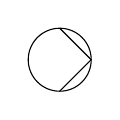
\begin{tikzpicture}[scale=0.8,transform shape]
%Pump
\draw (0,0) circle (0.5);
\draw (0.5,0) -- (0,0.5);
\draw (0.5,0) -- (0,-0.5);
\addvmargin{4mm}
\end{tikzpicture}

                  & Pump                          \\ \hline
      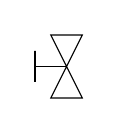
\begin{tikzpicture}[scale=0.8,transform shape]
%man-valve
\node(n1) at (0.25,2) {};
\node(n2) at (-0.25,2) {};
\node(n3) at (0.25,1) {};
\node(n4) at (-0.25,1) {};
\node(n5) at (0,1.5) {};
\node(n6) at (-0.5,1.75) {};
\node(n7) at (-0.5,1.25) {};
\draw(n1.center)--(n2.center)--(n3.center)--(n4.center)--(n1.center)--(n2.center);
\draw(n5.center)-|(n6.center)--(n7.center);
\addvmargin{4mm}
\end{tikzpicture}

          & Manual valve                  \\ \hline
      \tikzset{evalve/.style={draw, circle, inner sep=0pt, text width=3mm, align=center}}
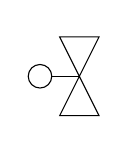
\begin{tikzpicture}
%elec-valve
\node(n1) at (4.25,2) {};
\node(n2) at (3.75,2) {};
\node(n3) at (4.25,1) {};
\node(n4) at (3.75,1) {};
\node(n5) at (4,1.5) {};
\node(n6) at (3.5,1.5) [evalve] {};
\draw(n1.center)--(n2.center)--(n3.center)--(n4.center)--(n1.center)--(n2.center);
\draw(n5.center)--(n6);
\addvmargin{4mm}
\end{tikzpicture}

            & Electronic valve              \\ \hline
      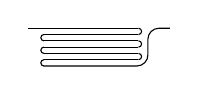
\begin{tikzpicture}[scale=0.8,transform shape]
%pipe
%right arcs
\draw (2.5,3.5) arc (90:-90:0.05);
\draw (2.5,3.3) arc (90:-90:0.05);
\draw (2.5,3.1) arc (90:-90:0.05);
%left arcs
\draw (1,3.4) arc (90:270:0.05);
\draw (1,3.2) arc (90:270:0.05);
\draw (1,3) arc (90:270:0.05);
%lines
\draw(0.75,3.5) -- (2.5,3.5);
\draw(1,3.4) -- (2.5,3.4);
\draw(1,3.3) -- (2.5,3.3);
\draw(1,3.2) -- (2.5,3.2);
\draw(1,3.1) -- (2.5,3.1);
\draw(1,3) -- (2.5,3);
\draw[rounded corners](1,2.9) -- (2.65,2.9) -- (2.65,3.5) -- (3,3.5);
\addvmargin{4mm}
\end{tikzpicture}

                  & Pipe segment                  \\ \hline
      \tikzset{pressure/.style={draw, circle, inner sep=0pt, text width=4mm, align=center}}
\tikzset{difpres/.style={draw, circle, inner sep=0pt, text width=5mm, align=center}}
\tikzset{connect/.style={draw,circle, inner sep=0pt, text width=2mm, align=center,fill=black}}
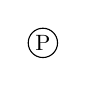
\begin{tikzpicture}[scale=0.8,transform shape]
%pressure sensor
\node(P1) at (0,0) [pressure] {P};
\addvmargin{4mm}
\end{tikzpicture}

       & Pressure sensor              \\ \hline
      \tikzset{pressure/.style={draw, circle, inner sep=0pt, text width=4mm, align=center}}
\tikzset{difpres/.style={draw, circle, inner sep=0pt, text width=5mm, align=center}}
\tikzset{connect/.style={draw,circle, inner sep=0pt, text width=2mm, align=center,fill=black}}

\begin{tikzpicture}[scale=0.8,transform shape]
%differential pressure sensor
\node(DP1) at (-2,0) [difpres] {DP};
\addvmargin{4mm}
\end{tikzpicture}

         & Differential pressure sensor  \\ \hline
      \begin{tikzpicture}[scale=0.8,transform shape]
%GND
\draw(-0.3,-2.5)--(0.3,-2.5);
\draw(-0.15,-2.6)--(0.15,-2.6);
\draw(0,-2.5)--(0,-2);
\addvmargin{4mm}
\end{tikzpicture}

                   & Gnd                           \\ \hline
    \end{tabular}
    \captionof{table}{Symbol and name for component in the water network.}  
    \label{tab:sys_comp_overview}
  \end{minipage}
\end{figure}



\section{System Graph}
\label{systemgraph}
\begin{figure}[H]
\centering
%\documentclass{article}

% example taken from 
% http://www.guitex.org/home/images/doc/GuideGuIT/introingtikz.pdf

\usepackage {tikz}
\usepackage{rotating}
\usetikzlibrary {positioning}



%\usepackage {xcolor}
\definecolor {processblue}{cmyk}{0.96,0,0,0}
\begin {document}
\begin{sidewaysfigure}[htb]
\begin {center}
\begin {tikzpicture}[-latex ,auto ,node distance =4 cm and 8cm ,on grid ,
semithick ,
state/.style ={ draw,shape=circle}]
\node[circle,fill,inner sep=3pt,label=below right:$n_4$] (A) at (0,0) {};
\node[circle,fill,inner sep=3pt,label=right:$n_8$] (B) at (0,4) {};
\node[circle,fill,inner sep=3pt,label=below right:$n_9$] (C) at (0,8) {};
\path (A) edge  node[right] {$e$} (B);
\path (B) edge  node[right] {$e$} (C);
\node[circle,fill,inner sep=3pt,label=right:$n_{10}$] (G) at (2,11) {};
\node[circle,fill,inner sep=3pt,label=right:$n_{11}$] (H) at (-1,10) {};
\node[circle,fill,inner sep=3pt,label=right:$n_{12}$] (I) at (-1,12) {};
\path (C) edge  node[right] {$e$} (G);
\path (C) edge  node[right] {$e$} (H);
\path (H) edge  node[right] {$e$} (I);



%
\node[circle,fill,inner sep=3pt,label=below right:$n_5$] (D) at (8,0) {};
\node[circle,fill,inner sep=3pt,label=right:$n_{13}$] (E) at (8,4) {};
\node[circle,fill,inner sep=3pt,label=right:$n_{14}$] (F) at (8,8) {};
\path (D) edge  node[right] {$e$} (E);
\path (E) edge  node[right] {$e$} (F);
\node[circle,fill,inner sep=3pt,label=right:$n_{15}$] (J) at (9,11) {};
\node[circle,fill,inner sep=3pt,label=right:$n_{16}$] (K) at (7,10) {};
\node[circle,fill,inner sep=3pt,label=right:$n_{17}$] (L) at (6,12) {};
\path (F) edge  node[right] {$e$} (J);
\path (F) edge  node[right] {$e$} (K);
\path (K) edge  node[right] {$e$} (L);

\node[circle,fill,inner sep=3pt,label=above:$n_{1}$] (M) at (4,14) {};

\path (A) edge  node[below] {$e$} (D);
\path (F) edge  node[below] {$e$} (C);
\path (G) edge [bend right = -15] node[below =0.15 cm] {$e$} (M);
\path (L) edge [bend left = -15] node[below =0.15 cm] {$e$} (M);
\path (I) edge [bend right = -15] node[below =0.15 cm] {$e$} (M);
\path (J) edge [bend left = -15] node[below =0.15 cm] {$e$} (M);


\node[circle,fill,inner sep=3pt,label=above:$n_{3}$] (N) at (-3,0) {};
\node[circle,fill,inner sep=3pt,label= above right:$n_{2}$] (O) at (-8,2) {};
\node[circle,fill,inner sep=3pt,label= above left :$n_{18}$] (P) at (-4,6) {};

\path (A) edge  node[below] {$e$} (N);
\path (P) edge [bend right = -50] node[below =0.15 cm] {$e$} (M);
\path (O) edge [bend right = -50] node[below =0.15 cm] {$e$} (M);
\path (N) edge  node[below] {$e$} (O);
\path (N) edge  node[right] {$e$} (P);


\node[circle,fill,inner sep=3pt,label=above right:$n_{6}$] (Q) at (11,0) {};
\node[circle,fill,inner sep=3pt,label=above right :$n_{7}$] (R) at (14,6) {};
\path (D) edge  node[below] {$e$} (Q);
\path (Q) edge  node[below right ] {$e$} (R);
\path (R) edge [bend left = -40] node[below =0.15 cm] {$e$} (M);
\path (N) edge [bend left = -20] node[below =0.15 cm] {$e$} (Q);




\end{tikzpicture}
\end{center}
\end{sidewaysfigure}

\end{document}
 
\resizebox{1\linewidth}{!}{\documentclass{article}

% example taken from 
% http://www.guitex.org/home/images/doc/GuideGuIT/introingtikz.pdf

\usepackage {tikz}
\usepackage{rotating}
\usetikzlibrary {positioning}



%\usepackage {xcolor}
\definecolor {processblue}{cmyk}{0.96,0,0,0}
\begin {document}
\begin{sidewaysfigure}[htb]
\begin {center}
\begin {tikzpicture}[-latex ,auto ,node distance =4 cm and 8cm ,on grid ,
semithick ,
state/.style ={ draw,shape=circle}]
\node[circle,fill,inner sep=3pt,label=below right:$n_4$] (A) at (0,0) {};
\node[circle,fill,inner sep=3pt,label=right:$n_8$] (B) at (0,4) {};
\node[circle,fill,inner sep=3pt,label=below right:$n_9$] (C) at (0,8) {};
\path (A) edge  node[right] {$e$} (B);
\path (B) edge  node[right] {$e$} (C);
\node[circle,fill,inner sep=3pt,label=right:$n_{10}$] (G) at (2,11) {};
\node[circle,fill,inner sep=3pt,label=right:$n_{11}$] (H) at (-1,10) {};
\node[circle,fill,inner sep=3pt,label=right:$n_{12}$] (I) at (-1,12) {};
\path (C) edge  node[right] {$e$} (G);
\path (C) edge  node[right] {$e$} (H);
\path (H) edge  node[right] {$e$} (I);



%
\node[circle,fill,inner sep=3pt,label=below right:$n_5$] (D) at (8,0) {};
\node[circle,fill,inner sep=3pt,label=right:$n_{13}$] (E) at (8,4) {};
\node[circle,fill,inner sep=3pt,label=right:$n_{14}$] (F) at (8,8) {};
\path (D) edge  node[right] {$e$} (E);
\path (E) edge  node[right] {$e$} (F);
\node[circle,fill,inner sep=3pt,label=right:$n_{15}$] (J) at (9,11) {};
\node[circle,fill,inner sep=3pt,label=right:$n_{16}$] (K) at (7,10) {};
\node[circle,fill,inner sep=3pt,label=right:$n_{17}$] (L) at (6,12) {};
\path (F) edge  node[right] {$e$} (J);
\path (F) edge  node[right] {$e$} (K);
\path (K) edge  node[right] {$e$} (L);

\node[circle,fill,inner sep=3pt,label=above:$n_{1}$] (M) at (4,14) {};

\path (A) edge  node[below] {$e$} (D);
\path (F) edge  node[below] {$e$} (C);
\path (G) edge [bend right = -15] node[below =0.15 cm] {$e$} (M);
\path (L) edge [bend left = -15] node[below =0.15 cm] {$e$} (M);
\path (I) edge [bend right = -15] node[below =0.15 cm] {$e$} (M);
\path (J) edge [bend left = -15] node[below =0.15 cm] {$e$} (M);


\node[circle,fill,inner sep=3pt,label=above:$n_{3}$] (N) at (-3,0) {};
\node[circle,fill,inner sep=3pt,label= above right:$n_{2}$] (O) at (-8,2) {};
\node[circle,fill,inner sep=3pt,label= above left :$n_{18}$] (P) at (-4,6) {};

\path (A) edge  node[below] {$e$} (N);
\path (P) edge [bend right = -50] node[below =0.15 cm] {$e$} (M);
\path (O) edge [bend right = -50] node[below =0.15 cm] {$e$} (M);
\path (N) edge  node[below] {$e$} (O);
\path (N) edge  node[right] {$e$} (P);


\node[circle,fill,inner sep=3pt,label=above right:$n_{6}$] (Q) at (11,0) {};
\node[circle,fill,inner sep=3pt,label=above right :$n_{7}$] (R) at (14,6) {};
\path (D) edge  node[below] {$e$} (Q);
\path (Q) edge  node[below right ] {$e$} (R);
\path (R) edge [bend left = -40] node[below =0.15 cm] {$e$} (M);
\path (N) edge [bend left = -20] node[below =0.15 cm] {$e$} (Q);




\end{tikzpicture}
\end{center}
\end{sidewaysfigure}

\end{document}
}
\end{figure}

\section{Spanning Tree}
\label{spanningtree}
\begin{figure}[H]
\centering
%
%\usepackage {tikz}
%\usepackage{rotating}
%\usepackage{amsmath}
%\usetikzlibrary {positioning}


%\usepackage {xcolor}
\begin{turn}{90}
\begin{tikzpicture}[-latex ,auto ,node distance =4 cm and 8cm ,on grid ,
semithick ,
state/.style ={ draw,shape=circle}]

\node[circle,fill,inner sep=3pt,label=below right:$n_4$] (A) at (0,0) {};
\node[circle,fill,inner sep=3pt,label=right:$n_8$] (B) at (0,4) {};
\node[circle,fill,inner sep=3pt,label=below right:$n_9$] (C) at (0,8) {};
\path (A) edge  node[right] {$e_9 c_{18}$} (B);
\path (B) edge  node[right] {$e_{10}c_{19}$} (C);
\node[circle,fill,inner sep=3pt,label=right:$n_{10}$] (G) at (2,11) {};
\node[circle,fill,inner sep=3pt,label=right:$n_{11}$] (H) at (-1,10) {};
\node[circle,fill,inner sep=3pt,label=right:$n_{12}$] (I) at (-1,12) {};
\path (C) edge  node[right] {$e_{14}c_{23}$} (G);
\path (H) edge  node[right] {$e_{12}c_{21}$} (I);



%
\node[circle,fill,inner sep=3pt,label=below right:$n_5$] (D) at (8,0) {};
\node[circle,fill,inner sep=3pt,label=right:$n_{13}$] (E) at (8,4) {};
\node[circle,fill,inner sep=3pt,label=right:$n_{14}$] (F) at (8,8) {};
\path (D) edge  node[right] {$e_{16}c_{25}$} (E);
\path (E) edge  node[right] {$e_{17}c_{26}$} (F);
\node[circle,fill,inner sep=3pt,label=right:$n_{15}$] (J) at (9,11) {};
\node[circle,fill,inner sep=3pt,label=right:$n_{16}$] (K) at (7,10) {};
\node[circle,fill,inner sep=3pt,label=right:$n_{17}$] (L) at (6,12) {};
\path (F) edge  node[left] {$e_{18}c_{29}$} (K);
\path (K) edge  node[left] {$e_{19}c_{28}$} (L);

\node[circle,fill,inner sep=3pt,label=above:$n_{1}$] (M) at (4,14) {};

\path (G) edge [bend right = -15] node[below left =0.15 cm] {$e_{15}c_{24}$} (M);
\path (L) edge [bend left = -15] node[below left =0.15 cm] {$e_{20}c_{27}$} (M);
\path (I) edge [bend right = -15] node[below =0.15 cm] {$e_{13}c_{20}$} (M);
\path (J) edge [bend left = -15] node[below =0.15 cm] {$e_{22}c_{31}$} (M);


\node[circle,fill,inner sep=3pt,label=above right :$n_{3}$] (N) at (-3,0) {};
\node[circle,fill,inner sep=3pt,label= above right:$n_{2}$] (O) at (-8,2) {};
\node[circle,fill,inner sep=3pt,label= above left :$n_{18}$] (P) at (-4,6) {};

\path (P) edge [bend right = -50] node[below left =0.15 cm] {$e_{25}c_{33}$} (M);
\path (M) edge [bend left = -50] node[below =0.15 cm] {$e_1c_2$} (O);
\path (N) edge  node[right] {$e_{24}c_{32}$} (P);



\node[circle,fill,inner sep=3pt,label=above right:$n_{6}$] (Q) at (11,0) {};
\node[circle,fill,inner sep=3pt,label=above right :$n_{7}$] (R) at (14,6) {};
\path (R) edge  node[below right ] {$e_7 c_{14}$} (Q);
\path (M) edge [bend right = -40] node[below =0.15 cm] {$e_8 c_{16}$} (R);


\end{tikzpicture}
\end{turn}
%\end{sidewaysfigure}
 
\resizebox{0.9\linewidth}{!}{
%\usepackage {tikz}
%\usepackage{rotating}
%\usepackage{amsmath}
%\usetikzlibrary {positioning}


%\usepackage {xcolor}
\begin{turn}{90}
\begin{tikzpicture}[-latex ,auto ,node distance =4 cm and 8cm ,on grid ,
semithick ,
state/.style ={ draw,shape=circle}]

\node[circle,fill,inner sep=3pt,label=below right:$n_4$] (A) at (0,0) {};
\node[circle,fill,inner sep=3pt,label=right:$n_8$] (B) at (0,4) {};
\node[circle,fill,inner sep=3pt,label=below right:$n_9$] (C) at (0,8) {};
\path (A) edge  node[right] {$e_9 c_{18}$} (B);
\path (B) edge  node[right] {$e_{10}c_{19}$} (C);
\node[circle,fill,inner sep=3pt,label=right:$n_{10}$] (G) at (2,11) {};
\node[circle,fill,inner sep=3pt,label=right:$n_{11}$] (H) at (-1,10) {};
\node[circle,fill,inner sep=3pt,label=right:$n_{12}$] (I) at (-1,12) {};
\path (C) edge  node[right] {$e_{14}c_{23}$} (G);
\path (H) edge  node[right] {$e_{12}c_{21}$} (I);



%
\node[circle,fill,inner sep=3pt,label=below right:$n_5$] (D) at (8,0) {};
\node[circle,fill,inner sep=3pt,label=right:$n_{13}$] (E) at (8,4) {};
\node[circle,fill,inner sep=3pt,label=right:$n_{14}$] (F) at (8,8) {};
\path (D) edge  node[right] {$e_{16}c_{25}$} (E);
\path (E) edge  node[right] {$e_{17}c_{26}$} (F);
\node[circle,fill,inner sep=3pt,label=right:$n_{15}$] (J) at (9,11) {};
\node[circle,fill,inner sep=3pt,label=right:$n_{16}$] (K) at (7,10) {};
\node[circle,fill,inner sep=3pt,label=right:$n_{17}$] (L) at (6,12) {};
\path (F) edge  node[left] {$e_{18}c_{29}$} (K);
\path (K) edge  node[left] {$e_{19}c_{28}$} (L);

\node[circle,fill,inner sep=3pt,label=above:$n_{1}$] (M) at (4,14) {};

\path (G) edge [bend right = -15] node[below left =0.15 cm] {$e_{15}c_{24}$} (M);
\path (L) edge [bend left = -15] node[below left =0.15 cm] {$e_{20}c_{27}$} (M);
\path (I) edge [bend right = -15] node[below =0.15 cm] {$e_{13}c_{20}$} (M);
\path (J) edge [bend left = -15] node[below =0.15 cm] {$e_{22}c_{31}$} (M);


\node[circle,fill,inner sep=3pt,label=above right :$n_{3}$] (N) at (-3,0) {};
\node[circle,fill,inner sep=3pt,label= above right:$n_{2}$] (O) at (-8,2) {};
\node[circle,fill,inner sep=3pt,label= above left :$n_{18}$] (P) at (-4,6) {};

\path (P) edge [bend right = -50] node[below left =0.15 cm] {$e_{25}c_{33}$} (M);
\path (M) edge [bend left = -50] node[below =0.15 cm] {$e_1c_2$} (O);
\path (N) edge  node[right] {$e_{24}c_{32}$} (P);



\node[circle,fill,inner sep=3pt,label=above right:$n_{6}$] (Q) at (11,0) {};
\node[circle,fill,inner sep=3pt,label=above right :$n_{7}$] (R) at (14,6) {};
\path (R) edge  node[below right ] {$e_7 c_{14}$} (Q);
\path (M) edge [bend right = -40] node[below =0.15 cm] {$e_8 c_{16}$} (R);


\end{tikzpicture}
\end{turn}
%\end{sidewaysfigure}
}
\end{figure}

\section{Incidence Matrix}
\label{IncidenceSection}
%\todo{Vinkel! this matrix appears in a different page than the section title, Also with the cycle matrix}
%\begin{sidewaysfigure}
\vspace{4mm}
\begin{equation}
  \label{graph_nodes}
%\resizebox{0.6\hsize}{!}{
%\rotatebox{90}{$
\begin{adjustbox}{max width=\textwidth}$H
=
\left[
\begin{array}{*{26}c}
   $ 18x24$ & e2 & e3 & e4 & e5 & e6 & e11 & e21 & e23 & e1 & e7 & e8 & e9 & e10 & e12 & e13 & e14 & e15 & e16 & e17 & e18 & e19 & e20 & e22 & e24 & 
e25 \\
n1 & 0 & 0 & 0 & 0 & 0 & 0 & 0 & 0 & 1 & 0 & 1 & 0 & 0 & 0 & -1 & 0 & -1 & 0 & 0 & 0 & 0 & -1 & -1 & 0 & -1 
\\
n2 & 1 & 0 & 0 & 0 & 0 & 0 & 0 & 0 & -1 & 0 & 0 & 0 & 0 & 0 & 0 & 0 & 0 & 0 & 0 & 0 & 0 & 0 & 0 & 0 & 0 
\\
n3 & -1 & 1 & 0 & 0 & -1 & 0 & 0 & 0 & 0 & 0 & 0 & 0 & 0 & 0 & 0 & 0 & 0 & 0 & 0 & 0 & 0 & 0 & 0 & 1 & 0 
\\
n4 & 0 & -1 & 1 & 0 & 0 & 0 & 0 & 0 & 0 & 0 & 0 & 1 & 0 & 0 & 0 & 0 & 0 & 0 & 0 & 0 & 0 & 0 & 0 & 0 & 0
\\
n5 & 0 & 0 & -1 & -1 & 0 & 0 & 0 & 0 & 0 & 0 & 0 & 0 & 0 & 0 & 0 & 0 & 0 & 1 & 0 & 0 & 0 & 0 & 0 & 0 & 0 
\\
n6 & 0 & 0 & 0 & 1 & 1 & 0 & 0 & 0 & 0 & -1 & 0 & 0 & 0 & 0 & 0 & 0 & 0 & 0 & 0 & 0 & 0 & 0 & 0 & 0 & 
0 \\
n7 & 0 & 0 & 0 & 0 & 0 & 0 & 0 & 0 & 0 & 1 & -1 & 0 & 0 & 0 & 0 & 0 & 0 & 0 & 0 & 0 & 0 & 0 & 0 & 0 & 0 
\\
n8 & 0 & 0 & 0 & 0 & 0 & 0 & 0 & 0 & 0 & 0 & 0 & -1 & 1 & 0 & 0 & 0 & 0 & 0 & 0 & 0 & 0 & 0 & 0 & 0 & 0 
\\
n9 & 0 & 0 & 0 & 0 & 0 & 1 & 0 & 1 & 0 & 0 & 0 & 0 & -1 & 0 & 0 & 1 & 0 & 0 & 0 & 0 & 0 & 0 & 0 & 0 & 0 
\\
n10 & 0 & 0 & 0 & 0 & 0 & 0 & 0 & 0 & 0 & 0 & 0 & 0 & 0 & 0 & 0 & -1 & 1 & 0 & 0 & 0 & 0 & 0 & 0 & 0 & 
0\\
n11 & 0 & 0 & 0 & 0 & 0 & -1 & 0 & 0 & 0 & 0 & 0 & 0 & 0 & 1 & 0 & 0 & 0 & 0 & 0 & 0 & 0 & 0 & 0 & 0 & 0 
\\
n12 & 0 & 0 & 0 & 0 & 0 & 0 & 0 & 0 & 0 & 0 & 0 & 0 & 0 & -1 & 1 & 0 & 0 & 0 & 0 & 0 & 0 & 0 & 0 & 0 & 0 
\\
n13  &  0 & 0 & 0 & 0 & 0 & 0 & 0 & 0 & 0 & 0 & 0 & 0 & 0 & 0 & 0 & 0 & 0 & -1 & 1 & 0 & 0 & 0 & 0 & 0 & 0 
\\
n14 & 0 & 0 & 0 & 0 & 0 & 0 & 1 & -1 & 0 & 0 & 0 & 0 & 0 & 0 & 0 & 0 & 0 & 0 & -1 & 1 & 0 & 0 & 0 & 0 & 0 
\\
n15 & 0 & 0 & 0 & 0 & 0 & 0 & -1 & 0 & 0 & 0 & 0 & 0 & 0 & 0 & 0 & 0 & 0 & 0 & 0 & 0 & 0 & 0 & 1 & 0 & 0 
\\
n16 & 0 & 0 & 0 & 0 & 0 & 0 & 0 & 0 & 0 & 0 & 0 & 0 & 0 & 0 & 0 & 0 & 0 & 0 & 0 & -1 & 1 & 0 & 0 & 0 & 0 
\\
n17 & 0 & 0 & 0 & 0 & 0 & 0 & 0 & 0 & 0 & 0 & 0 & 0 & 0 & 0 & 0 & 0 & 0 & 0 & 0 & 0 & -1 & 1 & 0 & 0 & 0 
\\
n18 & 0 & 0 & 0 & 0 & 0 & 0 & 0 & 0 & 0 & 0 & 0 & 0 & 0 & 0 & 0 & 0 & 0 & 0 & 0 & 0 & 0 & 0 & 0 & -1 & 1 


\end{array}
\right]$% }}
\end{adjustbox}
\end{equation}

\section{Cycle Matrix}
\label{CycleAppendix}
\vspace{4mm}

\begin{equation}
  \label{ComponentState}
%\resizebox{0.28\hsize}{!}{
%\rotatebox{90}{$
\begin{adjustbox}{max width=\textwidth}$B
=
\left[
\begin{array}{*{25}c}

1 & 0 & 0 & 0 & 0 & 0 & 0 & 0 & 1 & 0 & 0 & 0 & 0 & 0 & 0 & 0 & 0 & 0 & 0 & 0 & 0 & 0 & 0 & 1 & 1
 \\
  0 & 1 & 0 & 0 & 0 & 0 & 0 & 0 & 0 & 0 & 0 & 1 & 1 & 0 & 0 & 1 & 1 & 0 & 0 & 0 & 0 & 0 & 0   & -1   & -1
 \\
  0 & 0 & 1 & 0 & 0 & 0 & 0 & 0 & 0 & 0 & 0   & -1  &  -1 & 0 & 0   & -1  &  -1 & 1 & 1 & 1 & 1 & 1 & 0 & 0 & 0
 \\
  0 & 0 & 0 & 1 & 0 & 0 & 0 & 0 & 0 & 1 & 1 & 0 & 0 & 0 & 0 & 0 & 0 & 1 & 1 & 1 & 1 & 1 & 0 & 0 & 0
 \\
  0 & 0 & 0 & 0 & 1 & 0 & 0 & 0 & 0 & 1 & 1 & 0 & 0 & 0 & 0 & 0 & 0 & 0 & 0 & 0 & 0 & 0 & 0 & 1 & 1
 \\
  0 & 0 & 0 & 0 & 0 & 1 & 0 & 0 & 0 & 0 & 0 & 0 & 0 & 1 & 1  &  -1  &  -1 & 0 & 0 & 0 & 0 & 0 & 0 & 0 & 0
 \\
  0 & 0 & 0 & 0 & 0 & 0 & 1 & 0 & 0 & 0 & 0 & 0 & 0 & 0 & 0 & 0 & 0 & 0 & 0  &  -1  &  -1   & -1 & 1 & 0 & 0
 \\
 0 & 0 & 0 & 0 & 0 & 0 & 0 & 1 & 0 & 0 & 0 & 0 & 0 & 0 & 0   & -1    &-1 & 0 & 0 & 1 & 1 & 1 & 0 & 0 & 0
  
\end{array}
\right]$ %} }
\end{adjustbox}
\end{equation}
\vspace{-10mm}

\section{Mapping matrices}
\label{MappingAppendix}

\vspace{5mm}


\[
G=\left[\begin{array}{*{2}c}
0 & 0 \\
0 & 0 \\ 
0 & 0 \\ 
0 & 0 \\
0 & 0 \\
0 & 0 \\ 
0 & 0 \\ 
0 & 0 \\
1 & 0 \\
0 & 0 \\ 
0 & 1 \\ 
0 & 0 \\
0 & 0 \\
0 & 0 \\ 
0 & 0 \\ 
0 & 0 \\
0 & 0 \\
0 & 0 \\ 
0 & 0 \\ 
0 & 0 \\
0 & 0 \\
0 & 0 \\ 
0 & 0 \\ 
0 & 0 
  \end{array}\right]
\qquad
G_p=\left[\begin{array}{*{8}c}
0 & 0 & 0 & 0 & 0 & 0 & 0 & 0 
 \\
0 & 0 & 0 & 0 & 0 & 0 & 0 & 0 
 \\
0 & 0 & 0 & 0 & 0 & 0 & 0 & 0 
 \\
 0 & 0 & 0 & 0 & 0 & 0 & 0 & 0 
 \\
 0 & 0 & 0 & 0 & 0 & 0 & 0 & 0 
 \\
 0 & 0 & 0 & 0 & 0 & 0 & 0 & 0 
 \\
 0 & 0 & 0 & 0 & 0 & 0 & 0 & 0 
 \\
 0 & 0 & 0 & 0 & 0 & 0 & 0 & 0 
 \\
 0 & 0 & 0 & 0 & 1 & 0 & 0 & 0 
 \\
 0 & 0 & 0 & 0 & 0 & 0 & 0 & 0 
 \\
 0 & 0 & 0 & 0 & 0 & 1 & 0 & 0 
 \\
 0 & 0 & 0 & 0 & 0 & 0 & 1 & 0 
 \\
 0 & 0 & 0 & 0 & 0 & 0 & 0 & 0 
 \\
 0 & 0 & 0 & 0 & 0 & 0 & 0 & 0 
 \\
 0 & 0 & 0 & 0 & 0 & 0 & 0 & 0 
 \\
 0 & 0 & 0 & 0 & 0 & 0 & 0 & 0 
 \\
 0 & 0 & 0 & 0 & 0 & 0 & 0 & 0 
 \\
 0 & 0 & 0 & 0 & 0 & 0 & 0 & 1
 \\
 0 & 0 & 0 & 0 & 0 & 0 & 0 & 0 
 \\
 0 & 0 & 0 & 0 & 0 & 0 & 0 & 0 
 \\
 0 & 0 & 0 & 0 & 0 & 0 & 0 & 0 
 \\
 0 & 0 & 0 & 0 & 0 & 0 & 0 & 0 
 \\
 0 & 0 & 0 & 0 & 0 & 0 & 0 & 0 
 \\
 0 & 0 & 0 & 0 & 0 & 0 & 0 & 0
  \end{array}\right]
\]


%\pagebreak
%
%\section{Pipe Jacobian matrix}
%\label{PipeJacobianAppendix}
%\begin{equation}
%\frac{\partial{\lambda(\pmb{{B_1^{T}}}\pmb{z})}}{{\partial{\pmb{{B_1^{T}}}\pmb{z}}}}_{|\pmb{\bar{z}}}
%=
%\left[
%\begin{array}{*{8}c}
%\frac{\partial{\lambda(\pmb{{B_{1;1}^{T}}}\pmb{z})}}{{\partial{\pmb{{B_1^{T}}}\pmb{z}}}}_{|\bar{z}} & 0 & 0 & 0 & 0 & 0 & 0 & 0 
% \\
%0 & 0 & 0 & 0 & 0 & 0 & 0 & 0 
% \\
%0 & 0 & 0 & 0 & 0 & 0 & 0 & 0 
% \\
% 0 & 0 & 0 & 0 & 0 & 0 & 0 & 0 
% \\
% 0 & 0 & 0 & 0 & 0 & 0 & 0 & 0 
% \\
% 0 & 0 & 0 & 0 & 0 & 0 & 0 & 0 
% \\
% 0 & 0 & 0 & 0 & 0 & 0 & 0 & 0 
% \\
% 0 & 0 & 0 & 0 & 0 & 0 & 0 & 0 
% \\
% 0 & 0 & 0 & 0 & 1 & 0 & 0 & 0 
% \\
% 0 & 0 & 0 & 0 & 0 & 0 & 0 & 0 
% \\
% 0 & 0 & 0 & 0 & 0 & 1 & 0 & 0 
% \\
% 0 & 0 & 0 & 0 & 0 & 0 & 1 & 0 
%
%\end{array}
%\right]
%\pmb{{B_1^{T}}}
%\end{equation}





